\documentclass[12pt]{My_preprint}

\usetikzlibrary{arrows.meta,
                chains,
                positioning,
                shapes.geometric}
%%%%%%%%%%%%%%%%%%%%%%%%%%%%%%%%%%%%%%%%%%%%%%%%%%%%%%%%%%%%%%%%%%%%%%%%%%%%%%%
\newcommand{\size}{0.22\textwidth}
\newcommand{\avg}[1]{\left<#1\right>}
\renewcommand{\avg}[1]{\left<#1\right>}
\newcommand{\condavg}[1]{\left<#1 | \mathscr{C}_1\right>}
\newcommand{\Exp}[1]{\overline{\overline{#1}}}
\newcommand{\davg}[1]{\left<#1\right>_d}
\newcommand{\Iavg}[1]{\left<#1\right>_I}
\newcommand{\pavg}[1]{\avg{\delta_\alpha #1}}
% \newcommand{\pnavg}[1]{n\left<#1\right>_p}

\newcommand{\avgcond}[1]{\overline{#1}}
% \renewcommand{\avgcond}[1]{\left{#1}}
\newcommand{\kavg}[1]{\avgcond{#1}^k}
\newcommand{\cavg}[1]{\avgcond{#1}^c}
\newcommand{\Tavg}[1]{\avgcond{#1}^T}
\newcommand{\Xavg}[1]{\avgcond{#1}^X}
\newcommand{\TXavg}[1]{\Tavg{\Xavg{#1}}}
\newcommand{\pnnavg}[1]{\avgcond{#1}^{p}}
\newcommand{\pnavg}[1]{n_p\pnnavg{#1}}
\newcommand{\oneavg}[1]{\avgcond{#1}^1}
\newcommand{\twoavg}[1]{\avgcond{#1}^2}
\newcommand{\smallavg}[2]{\avgcond{#1}^{#2}}
\newcommand{\sym}[1]{\left(#1\right)^{\text{Sym}}}
\newcommand{\CC}{\mathscr{C}}
\newcommand{\PP}{\mathscr{P}}
\newcommand{\nstavg}[1]{\overline{#1}^\text{nst}}
\newcommand{\nstrelavg}[1]{\nstavg{#1}_\text{rel}}
\newcommand{\mavg}[1]{\left<#1\right>_m}
\newcommand{\gavg}[2][\gamma]{\left<#2\right>_{#1}}
\newcommand{\partials}[1]{\partial_{i_1}\partial_{i_2}\ldots\partial{i_{#1}}}
\newcommand{\partialp}[2]{ \prod_{m=#1}^{#2} \partial_{i_m}}
\newcommand{\hatpartialp}[2]{ \prod_{m=#1}^{#2} \hat{\partial}_{j_m}}
\newcommand{\hatpartialpi}[2]{ \prod_{m=#1}^{#2} \hat{\partial}_{i_m}}
\newcommand{\pri}[2]{ \prod_{m=#1}^{#2} r_{i_m}}
\newcommand{\prj}[2]{ \prod_{m=#1}^{#2} r_{j_m}}
\newcommand{\nablab}{\mathbf{\nabla}}
\newcommand{\nablabh}{\nablab}
\newcommand{\nablabhI}{\nablab_{||}}
\newcommand{\ddt}{\frac{d}{d t}}
\newcommand{\pddt}{\frac{\partial}{\partial t}}
\renewcommand{\pddt}{\partial_t}
\newcommand{\norm}[1]{\hat{#1}}
\newcommand{\Jump}[1]{\llbracket #1 \rrbracket \cdot \textbf{n} }

%%% Utiliser pour les commentaires
\newcommand{\JL}[1]{\color{red}#1\color{black}}
\newcommand{\SP}[1]{\color{green}#1\color{black}}
\newcommand{\tb}[1]{\color{blue}#1\color{black}}
\newcommand{\NF}[1]{\tb{#1}}

\renewcommand{\size}[1]{0.3\textwidth}
\newcommand{\expo}[2][n]{\frac{(-1)^#1}{#1!} \partialp{1}{#1} \pavg{\int_{\Omega_\alpha} \pri{1}{#1}#2 d\Omega}}
\newcommand{\expoU}[2][n]{\frac{(-1)^#1}{#1!} \partialp{1}{#1} \pavg{\textbf{u}_\alpha\int_{\Omega_\alpha} \pri{1}{#1}#2 d\Omega}}
\newcommand{\expoS}[2][n]{\frac{(-1)^#1}{#1!} \partialp{1}{#1} \pavg{\int_{\Sigma_\alpha} \pri{1}{#1}#2 d\Sigma}}


% \newcommand{\numref}[1]{\ref{#1}}
\renewcommand{\ref}[1]{\autoref{#1}}

%%%%%%%%%%%%%%%%%%%%%%%%%%%%%%% Title & Author %%%%%%%%%%%%%%%%%%%%%%%%%%%%%%%%


\title{Nearest particle statistics in rising monodisperse suspensions of drops}

\author[1,2]{Nicolas Fintzi}
\author[1]{Jean-Lou Pierson}
\author[2]{Stephane Popinet}
\affil[1]{IFP Energies Nouvelles, Rond-point de l’echangeur de Solaize, 69360 Solaize}
\affil[2]{Sorbonne Université, Institut Jean le Rond d’Alembert, 4 place Jussieu, 75252 PARIS CEDEX 05, France}
\normalmarginpar


\begin{document}

\maketitle

\begin{abstract}

\end{abstract}

\section{Introduction}
Even in the Stokes flow regime and in the limit of very dilute flows the calculation of the the sedimentation velocity of spherical inclusion is still a matter of research.  Batchelor in this seminal work showed by assuming that the particle where randomly distributed that the velocity of the particle was $U/U_0=1-\phi$, by making use oa re normalization technique to avoid the effect of non-convergin integral. This results has been extended to drops by wachollder and ... finding ... Over the past decades many experimental works have tried to find he relative motion between the particle and
the fluid phases result in microstructures affecting the sedimentation
velocity. En fiat cichocky en utilisant n-body formulation montre visiblement qu'il ya une vrai micro-strucutre. This question was raise first by Saffman whco by using the formalism of distribution showed the dramatic difference between the thrrre different configurations..."
Fait par wachholder etc As a result most of the study make use of the empirical correlation given by Richardson Zaki

\section{Computational methodology}
%\section{Numerical procedure and problem statement}
\subsection{Numerical method}

In this problem, the governing equations consist of the one-fluid formulation of the mass and momentum equation, with an additional transport equation for the dispersed phase indicator function. 
We recall their form here, 
\begin{align}
    \pddt \rho+ \div(\rho\textbf{u})
    &= 0,\\
    \label{eq:dt_urho}
    \pddt (\rho \textbf{u})
    + \div (\rho  \textbf{u} \textbf{u} - \bm\sigma)
    &= (\avg{\rho} - \rho)\textbf{g}
    + \textbf{f}_\gamma,\\
    \label{eq:dt_C}
    \pddt C + \textbf{u}\cdot\grad C  
    &= 0,
\end{align}
% \tb{mettre le link navier stokes solver et faire ca pour le reste }
which are the mass, momentum and colors function transport equation, respectively. 
The scalar fields $C$, represents the color function, which range between $0$ and $1$ to indicate the proportion of fluid and dispersed phase, respectively. 
We introduced the fluid velocity vector $\textbf{u}$ and the Newtonian stress tensor $\bm{\sigma} = -p \textbf{I} + \mu (\grad \textbf{u}+ \grad \textbf{u}^\dagger)$ where $p$ is the pressure fields and $^\dagger$ represents the transpose operator.
Note that the material properties, $\rho$ and $\mu$, take the value of the phases in presence, following the arithmetic average : $\rho = (1-C)\rho_f + C \rho_d$ and $\mu = (1-C)\mu_f + C \mu_d$. 
In our case the arithmetic mean turns out to perform better compared to the harmonic mean, which is often used to interpolate the viscosity for bubbly flows \citet{hidman2023assessing,innocenti2020direct}.
More details about this choice is provided in \ref{ap:validation} (\textit{Case 1.}). 
The capillary force is defined as, $\textbf{f}_\gamma =\textbf{n} \gamma \div \textbf{n} $, where \textbf{n} is the normal at the interface.
Following  \citep{bunner2002dynamics}, we incorporated the artificial body force term, $\avg{\rho}\textbf{g}$, on the right-hand side of \ref{eq:dt_urho}, to maintain a zero-averaged velocity throughout the entire numerical domain.  

To solve these equations we first initialized $125$ spherical droplets within a cubic domain with fully periodic boundary condition. 
We used the open source code \url{http///basilisk.fr} to discretize the governing equations in a multigrid solver. 
The Navier-Stokes equations are discretized with a centered scheme.
The two-phase flow solver uses the Volume of Fluid (VoF) method. 
The interfaces between the droplets and the carrier fluid is reconstructed using the Piecewise Linear Inter-face Calculation or PLIC method \citet[Chapter 5.]{tryggvason2011direct}.
Regarding the treatment of the surface tension force term we refer the reader to \citet{popinet2018numerical} for more details. 
The Basilisk solver has been validated extensively, in the framework of bubbly flow. 
Most of the previous studies \citep{hidman2023assessing,innocenti2020direct} recommend a grid definition of $\Delta/d \ge  30$, where $\Delta$ is the grid spacing. 
In \ref{ap:validation} we carried a mesh independence study and demonstrate that a grid spacing of $\Delta = d/30$ is also suitable in our context.
For readers seeking more detailed information about the solvers, we recommend the wiki pages : \href{http://basilisk.fr/src/navier-stokes/centered.h}{centered.h}, \href{http://basilisk.fr/src/tension.h}{tension.h} and \href{http://basilisk.fr/src/poissson.h}{poissson.h} where he can find the source code of the Navier-Stokes, surface tension and multigrid solver used in this work, respectively. 

With the VoF method droplets and bubbles may experience premature coalesce.
For a detailed discussion on this issue, see  \citet[Appendix B]{innocenti2020direct}.
However, in this work, it is imperative to conserve a specific (mono-disperse) population of droplets over time to accumulate sufficient statistics about the microstructure.
To tackle this issue we present in the next section a novel algorithm which prevent coalescence between droplets, while maintaining a reasonable cost. 






\subsection{The \texttt{no-coalescence.h} algorithm}

In previous studies various methods have been used to avoid coalescence. 
One method is to increase artificially the surface tension coefficient at the interface contact points, as demonstrated in the recent study of \citet{hidman2023assessing}.
% This method seems highly efficient, in terms of simplicity and computational expenses. 
However, it remains unclear if the physical behavior of the droplets interactions is well captured due to the introduction of artificial forces. 
Additionally, its applicability for denser emulsions, up to $\phi = 0.2$, remains uncertain. 
\citet{balcazar2015multiple} developed a multiple-marker level-set method to prevent coalescence, while \citet{zhang2021direct} used a multi-VoF method. 
The latter method consists in assigning to each droplet a different color function so  that the interfaces are reconstructed independently when droplets are in close contact.
Since the representations of the interfaces are independent, droplets in contact never coalesce.  
The latter method may be suitable for our objectives, however, it can be quite expensive as it requires solving a transport equation for each tracer, with one tracer assigned per droplet, meaning $125$ tracers in our case. 
\citet{karnakov2022computing} developed a multi-VoF method which requires a fixed number of tracers for an arbitrary number of droplets.
This approach allows multiple non-touching droplets to belong to the same field, which makes it more efficient than the previous study.
Although this approach shares the same basic principle with the one used here, i.e. coloring adjacent droplets with different colors to avoid coalescence, it differs in term of computational methods. 
In the following we present our methodology that as implemented in the \texttt{Basilisk} framework. 

The challenge here is to assign a tracer to every adjacent droplets to prevent numerical coalesce, while minimizing the number of tracers to reduce computational cost. 
This recalls the famous \textit{Four color map theorem} \citep{appel1977solution} which essentially states that : 
\enquote{every map can be color using only four colors, so that two neighboring region are different colors}. 
In our case, this theorem implies that for any 2D configuration only four VoF tracer are necessary to avoid coalescence\footnote{It is worth noting that for a bi-periodic domain, seven colors are required due to the torus-like topology.  }. 
Therefore, leveraging the \textit{Four color map theorem}, one might be able to significantly reduce the number of VoF tracers required.
Note however that the optimal coloring problem is originally a static problem that need to be solved only once. 
In our case, droplets move around over time thus transforming the static problem into a time-dependent problem. 
Furthermore finding the optimal coloring is known to be difficult (the problem is {\em NP-complete}) and solving it at each timestep would be too expensive.

Note also that in three-dimensions the \textit{Four color map theorem} has no equivalent.
For example, an arbitrary large number of rectangular blocks in 3D-space can all touch each other, requiring an arbitrary large number of colors to differentiate the adjacent blocks\citep{magnant2011coloring}. 
We are not aware of an extension of the coloring problem to arrangements of spheres in 3D. 
Nevertheless, it is reasonable to assume that the number of tracers required to avoid coalescence is significantly smaller than the number of droplets.
Consequently, since we cannot determine the optimal coloring configuration based on theoretical grounds, we opt to assign the tracers to each droplet following the empirical strategy detailed below.

The development of the \texttt{no-coalesce.h} algorithm was initiated in the PhD. thesis of \citet{mani2021numerical}.
The latest version of this algorithm can be found on the basilisk wiki page : \href{http://basilisk.fr/sandbox/fintzin/Rising-Suspenion/no-coalescence.h}{no-coalescence.h}.
Before  diving into a step-by-step description of this algorithm we need to introduce another key feature used in these simulations, which is the \href{http://basilisk.fr/src/tag.h}{tag.h} algorithm. 
It is an adaptation of the \textit{painter}'s algorithm, but optimized using the multigrid solver of \texttt{Basilisk}. 
Its purpose is to assign different scalars values to each cell belonging to different regions, with the regions being delimited by the different droplets' interfaces. 
For instance, on \ref{fig:images} (left) we can see two blue regions corresponding to two different drops.
We can notice that both are assigned with two different values, $1$ and $2$, which are identified using the \texttt{tag.h} algorithm. 
It is then straightforward to obtain the droplet properties, such as its center of mass, by carrying numerical integration on the VoF field considering only the cells having a specific tag value, which corresponds to a given droplet.  
% In general, we are able to differentiate droplets' domain, belonging to the same tracer thanks to the \texttt{tag.h} algorithm.


We define the $i^\text{th}$ color function as $C_i$ for $i =1,2,\ldots,N(t)$, where $N(t)$ is the total number of tracers used in a simulation at time $t$.
The color function introduced previously is now defined as, $C = \sum_{i=1}^{N(t)} C_i$. 
Note that $N(t)$ is time-dependent since the number of tracers may increase during the simulation as droplets get closer to one another.
The simplified workflow of the algorithm follows these four steps : 
\begin{enumerate}
    \item[\textit{Step 1}.] Check if within a tracer field $C_i$, the droplets are possibly too close to each other. 
    The \textit{near contact} criterion that determines if the droplets are too close is defined using a $5$ by $5$ cells stencil which verifies the following conditions : 
    (1) If the color function $C_i = 0$ at the center of the stencil. 
    (2) And if $C_i > 1$ for two opposite cells in the stencil. 
    In this case two different regions might be in close contact.
    A sketch of this situation is given in \ref{fig:criterion}.  
    \item[\textit{Step 2}.] 
    If (\textit{Step 1}.) is true for the tracer $C_i$, we must verify if we indeed identified two different regions in near contact, and not just a single region close to itself, such as in \ref{fig:diagram} (right). 
    Therefore at this step  we apply the \texttt{tag.h} algorithm.
    \item[\textit{Step 3}.] Re-use the \textit{near contact} criterion of (\textit{Step 1}.) by requiring in addition that the cells must belong to two different tag groups. 
    At this stage the situation in \ref{fig:criterion} (left) would be true, while the situation on \ref{fig:criterion} (right) would be false. 
    We therefore identified all the droplets / region that are indeed too close to each other. 
    \item[\textit{Step 4}.] 
    Find a new tracer field $C_n$, with which we could set the region/droplets that are in near contact. 
    At this stage, it is essential to identify the list of tracer $C_j$ already in contact with the region to be replaced. 
    For example, in \ref{fig:criterion} (left), the droplet on the right is clearly adjacent to a region with tracer $C_j$, in which case $C_n$ must satisfy $n \neq i,j$. 
    Therefore, any $n$ in $1, 2, \ldots, N(t)$ are suitable candidates as long as this situation is avoided. 
    If the droplet is already adjacent to every tracer $C_j$ in the simulation, for $j = 1, 2, \ldots, N(t)$, we create a new tracer $C_n$ with $n = N(t)+1$ and assign the drop to this tracer field.
\end{enumerate}
\begin{figure}
    \centering
    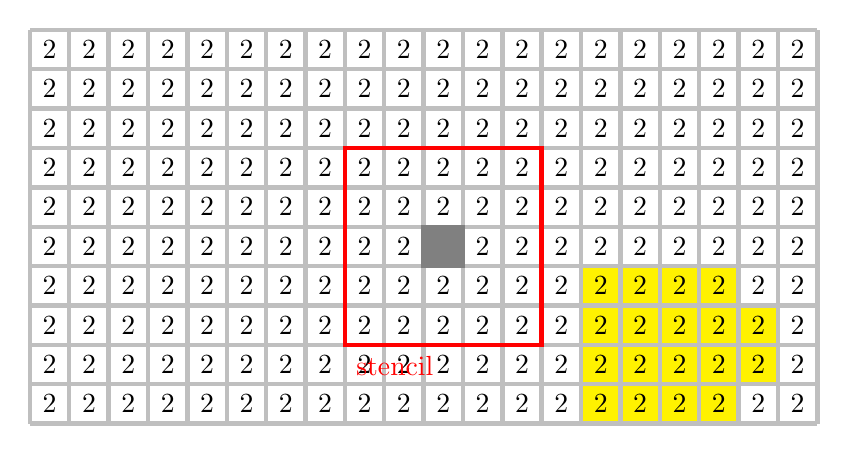
\begin{tikzpicture}[scale=0.5,ultra thick]
        % Define grid dimensions
        \def\nRows{10}
        \def\nCols{20}
        \pgfmathsetmacro\nRowsm{\nRows-1}
        \pgfmathsetmacro\nColsm{\nCols-1}

        \foreach \row in {0,...,\nRowsm} {
            \foreach \col in {0,...,\nColsm} {
                \pgfmathsetmacro\distance{veclen(\col-4.356, \row-2.65)};
                \pgfmathparse{\distance < 4 ? "blue" : "white"}
                \edef\colour{\pgfmathresult};
                \ifthenelse{\equal{\colour}{blue}}{                    
                    \fill[\colour!60!white] (\col, \row) rectangle ++(1,1);
                    \node (num) at (\col +0.5,\row+0.5){1};
                }
            }
        }

        \foreach \row in {0,...,\nRowsm} {
            \foreach \col in {0,...,\nColsm} {
                \pgfmathsetmacro\distance{veclen(\col-15, \row-6.2)};
                \pgfmathparse{\distance < 3.5 ? "blue" :"white"}
                \edef\colour{\pgfmathresult};
                \ifthenelse{\equal{\colour}{blue}}{
                    \fill[\colour!60!white] (\col, \row) rectangle ++(1,1);
                \node (num) at (\col +0.5,\row+0.5){2};
                }
            }
        }

        \foreach \row in {0,...,\nRowsm} {
            \foreach \col in {0,...,\nColsm} {
                \pgfmathsetmacro\distance{veclen(\col-15.62, \row-1.5)};
                \pgfmathparse{\distance < 2.5 ? "yellow" :"white"}
                \edef\colour{\pgfmathresult};
                \ifthenelse{\equal{\colour}{yellow}}{
                    \fill[\colour] (\col, \row) rectangle ++(1,1);
                    \node (num) at (\col +0.5,\row+0.5){2};
                }
            }
        }
        % Define grid size
        \pgfmathsetmacro\gridSize{1}
        
        \foreach \row in {0,...,\nRows} {
            \draw [gray!50] (0,\row*\gridSize) -- (\nCols*\gridSize,\row*\gridSize);
        }
        % Draw vertical grid lines
        \foreach \col in {0,...,\nCols} {
            \draw [gray!50] (\col*\gridSize,0) -- (\col*\gridSize,\nRows*\gridSize);
        }
        % Draw drop shape
        \draw[red] (8,2)node[below right]{stencil} rectangle +(5,5); % Draw the rectangular base
        \filldraw[gray] (10,4) rectangle +(1,1);
    \end{tikzpicture}    
    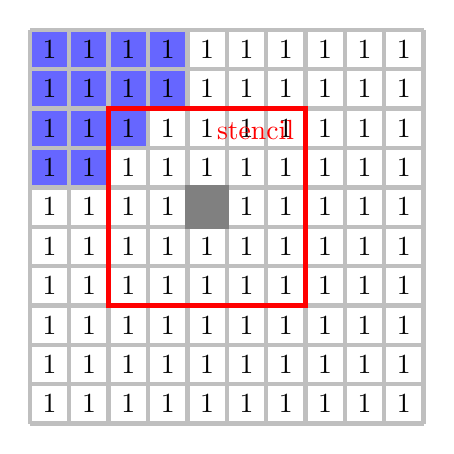
\begin{tikzpicture}[scale=0.5,ultra thick]
        % Define grid dimensions
        \def\nRows{10}
        \def\nCols{10}
        \pgfmathsetmacro\nRowsm{\nRows-1}
        \pgfmathsetmacro\nColsm{\nCols-1}

        \foreach \row in {0,...,\nRowsm} {
            \foreach \col in {0,...,\nColsm} {
                \pgfmathsetmacro\distance{veclen(\col, \row-2)};
                \pgfmathparse{\distance < 3.5 ? "blue" :"white"}
                \edef\colour{\pgfmathresult};
                \ifthenelse{\equal{\colour}{blue}}{
                    \fill[\colour!60!white] (\col, \row) rectangle ++(1,1);
                \node (num) at (\col +0.5,\row+0.5){1};
                }
            }
        }

        \foreach \row in {0,...,\nRowsm} {
            \foreach \col in {0,...,\nColsm} {
                \pgfmathsetmacro\distance{veclen(\col-7, \row-2)};
                \pgfmathparse{\distance < 3.5 ? "blue" :"white"}
                \edef\colour{\pgfmathresult};
                \ifthenelse{\equal{\colour}{blue}}{
                    \fill[\colour!60!white] (\col, \row) rectangle ++(1,1);
                    \node (num) at (\col +0.5,\row+0.5){1};
                }
            }
        }
        \foreach \row in {0,...,\nRowsm} {
            \foreach \col in {0,...,\nColsm} {
                \pgfmathsetmacro\distance{veclen(\col-5, \row)};
                \pgfmathparse{\distance < 3.5 ? "blue" :"white"}
                \edef\colour{\pgfmathresult};
                \ifthenelse{\equal{\colour}{blue}}{
                    \fill[\colour!60!white] (\col, \row) rectangle ++(1,1);
                    \node (num) at (\col +0.5,\row+0.5){1};
                }
            }
        }
        \foreach \row in {0,...,\nRowsm} {
            \foreach \col in {0,...,\nColsm} {
                \pgfmathsetmacro\distance{veclen(\col, \row-9)};
                \pgfmathparse{\distance < 3.5 ? "blue" :"white"}
                \edef\colour{\pgfmathresult};
                \ifthenelse{\equal{\colour}{blue}}{
                    \fill[\colour!60!white] (\col, \row) rectangle ++(1,1);
                    \node (num) at (\col +0.5,\row+0.5){1};
                }
            }
        }
        % Define grid size
        \pgfmathsetmacro\gridSize{1}
        
        \foreach \row in {0,...,\nRows} {
            \draw [gray!50] (0,\row*\gridSize) -- (\nCols*\gridSize,\row*\gridSize);
        }
        % Draw vertical grid lines
        \foreach \col in {0,...,\nCols} {
            \draw [gray!50] (\col*\gridSize,0) -- (\col*\gridSize,\nRows*\gridSize);
        }
        % Draw drop shape
        \draw[red] (2,3) rectangle +(5,5)node[below left]{stencil}; % Draw the rectangular base
        \filldraw[gray] (4,5) rectangle +(1,1);
    \end{tikzpicture}    
    \caption{Sketch of two situations were the \textit{near contact} criterion is true. 
    The background grid represents the cells within the numerical domain. 
    The dark blue area represents the cells where $C_i > 0$.
    The yellow area represents the cells where the tracer $C_j > 0$ for $j\neq i$. 
    The numbers represent the values of the $Tag$ scalar field within each tracer.
    The $5$ by $5$ cells red rectangle represents the stencil zone which iterates over all cells of the domain.  
    %  where the center of the stencil (gray square) must respect $C_i = 0$. 
    (left) Two droplets in contact since we have two opposite cells in the stencil with $C_i > 0$ and $C_i=0$ at the center.
    And the mentioned cells belong to two different regions so that (\textit{Step 3}) is also validated.  
    (right) A near contact is observed since we have two opposite cells in the stencil with $C_i > 0$ and $C_i=0$ at the center, however in this case we do not verify the second criterion of \textit{Step 3} which requires two different tags values. 
    }
    \label{fig:criterion}
\end{figure}
These four steps are executed at each simulation time step and for each tracer $C_i$ with $i = 1, 2, \ldots, N(t)$.
Following this procedure, we ensure that all adjacent droplets are using different tracers, which ultimately prevents coalescence. 

Having $N(t)$ tracers requires some modifications to the aforementioned governing equations. 
Specifically, instead of solving \ref{eq:dt_C}, we solve $N(t)$ transport equations, one for each $C_i$.
Likewise, the surface tension force is computed as the sum of the contributions from each $C_i$ and reads
\begin{align*}
    \pddt C_i + \textbf{u}\cdot\grad C_i = 0,
    \ \  \ \ \forall i = 1,2,\ldots N(t),\\
    \textbf{f}_\gamma 
    = \sum_{i=0}^{N(t)} \gamma \kappa_i \grad C_i
\end{align*}
where $\kappa_i$ is the numerical approximation of the curvature of the interface of field $C_i$, which is computed following the same method employed for a single tracer. 

\ref{fig:diagram} (left) shows a snapshot of a simulation at an arbitrary time $t^* = 100 \sqrt{g/d}$. 
The droplet interfaces are colored by the indices of their respective tracer. 
In this simulation at that time, no more than 3 colors are needed to avoid coalescence.
On \ref{fig:diagram} (right) we display the value of $N(t)$ in term of the dimensionless simulation time for various volume fractions $\phi$ at $Ga = 50$ and  $\lambda = 1$. 
We observe that for the entire simulation, no more than 3 tracers were needed for the dilute emulsion ($\phi = 0.01$) and up to 7 for the denser regime ($\phi = 0.2$). 
Although our algorithm might not be optimized, it brings sufficient efficiency for our needs. 
Indeed, \ref{tab:performance} reports the time spent by each function during a simulation. 
It is observed that the \texttt{no-coalesce.h} algorithm accounts for approximately $4\%$ of the total computational time of a simulation. 
As for the \texttt{tag.h} algorithm, its cost is around $2\%$, which is also reasonable.
In comparison, the \texttt{poisson.h} solver is about $13\%$ of the simulation time. 
The advection of VoF tracers is about $7\%$ which is relatively high but still reasonable.
To reduce the cost related to the \texttt{no-coalesce.h} algorithm we believe that further developments, which are referenced at \href{http://basilisk.fr/sandbox/fintzin/Rising-Suspenion/no-coalescence.h}{no-coalescence.h}, are still doable and could be useful for future studies.
\begin{figure}[h!]
    \centering
    \begin{tikzpicture}
    \node (img) at (0,0) {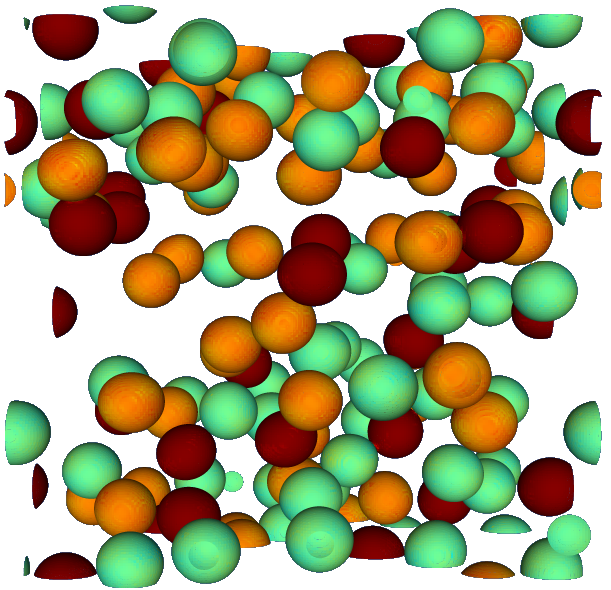
\includegraphics[width = 0.4\textwidth]{image/VoF2.png}};
    \node (img) at (0.4\textwidth,-0.01\textwidth) {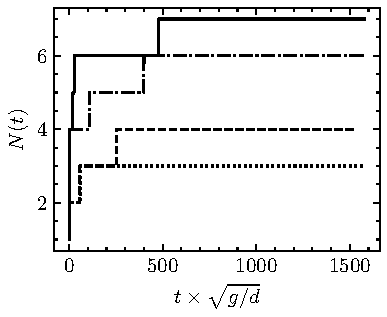
\includegraphics[width = 0.4\textwidth]{image/HOMOGENEOUS_NEW/CA/NVoF_vs_t_Ga_50_l_1.pdf}};
    \end{tikzpicture}
    \caption{
    (left) Snapshot of a DNS with $\phi = 0.05$, $\lambda = 1$, $Ga = 50$ with the interface of the droplets colored by the index of the tracers.
    (right) Number of tracers $N(t)$ as a function the dimensionless time.
    Four different volume fractions are displayed : (dotted line) $\phi = 0.01$, (dashed line) $\phi = 0.05$ (dash dotted line) $\phi = 0.1$ (solid line) $\phi = 0.2$ at $Ga = 50$ and $\lambda = 1$. 
    }
    \label{fig:diagram}
\end{figure}


In order to validate our numerical methodology, we have compared our numerical results to the experiments of \citet{mohamed2003drop} where they experimentally study the impact of a single drop on a flat interface of the same fluid. %, while recording the positions of the interfaces.
It is found that the multi-VoF method captures remarkably well the position of interfaces, even with a poor description of the liquid film between these interfaces.
Additionally, we argue that the mesh independence study conducted in \ref{ap:validation} (Case 3) substantiates the accuracy of the DNS, as the dynamics of interaction do converge with  reasonable errors for a grid resolution of $\Delta/d = 30$. 
Overall, we used an optimized multi-VoF method, enabling us to perform DNS with a maximum of 7 tracers in the densest scenario.
 






%\section{Preliminary tests}
%\label{sec:preliminary}


This section outlines the approach employed for performing simulations to achieve statistically steady states in the context of a rising mono-disperse suspension of droplets within a fully periodic domain.
We start by presenting the relevant physical parameters, followed by an overview of the numerical methods employed.
Finally, we detail the methodology implemented for collecting statistical data on microstructure, which will be presented in the following sections.

%In this section we expose the strategy employed to conduct statistically steady state simulations of rising mono-disperse suspension of droplets in a fully periodic domain. 
%We start by introducing the physical parameter, followed by a description of the numerical methods.
%Lastly, we detail the methodology adopted to collect statistics about microstructure, which are presented in the next sections.

%The source code used to perform the DNS is entirely open source.
%The simulations are running within the \texttt{Basilisk C} framework, (see \href{http://basilisk.fr}{basilisk.fr}), which is an extension of the C programming language, adapted for the solution of partial differential equations on Cartesian meshes. 
%Note that this section is complemented by the wiki page, \href{http://basilisk.fr/sandbox/fintzin/Rising-Suspension/RS.c}{RS.c}, where the reader can access the source code used to conduct the DNS, as well as comments and notes to help comprehension. 

\subsection{Problem statement}

We investigate numerically the dynamics of homogeneous mono-disperse emulsions subject to buoyancy forces in a fully periodic domain. 
The dispersed and continuous phases are considered Newtonian fluids defined by viscosity $\mu_d$ (resp. $\mu_f$) and density $\rho_d$ (resp. $\mu_f$).
Throughout this work, the subscript $_d$ and $_f$ indicate properties belonging to the dispersed and continuous phases, respectively. 
The interface between both fluids is considered infinitely thin, free of impurities, and characterized by a constant surface tension $\gamma$. %with a coefficient  is assumed. 
The density and viscosity will be considered constant in each phase.
In dimensionless form, this problem is completely characterized by six dimensionless parameters:  the viscosity and density ratio, $\lambda = \mu_d / \mu_f$ and $\zeta = \rho_d / \rho_f$,  
the \textit{Galileo} number, 
\begin{equation*}
    Ga =\frac{\sqrt{\rho_f(\rho_f - \rho_d) g d^3}}{\mu_f},
\end{equation*}
the \textit{Bond} number, 
\begin{equation*}
    Bo =\frac{(\rho_f - \rho_d) g d^2}{\gamma},
\end{equation*}
the number of droplets per domain $N_b$, and the dispersed phase volume fraction $\phi$. 
Here, $d$ represents the diameter of a sphere with the same volume as the droplets and $g$ denotes the acceleration of gravity.
The \textit{Galileo} number measures the strength of the buoyancy forces relative to the viscous forces, whereas the \textit{Bond} number evaluates the ratio between buoyancy and capillary forces. 

%To provide a brief overview of the range of interest for these numbers in an industrial context, let us consider the example of a vegetable oil/water system.
%In most liquid-liquid system encountered in industrial processes the diameter of the droplets lies in the range $d = [50 \mu \text{m}, 3 \text{mm}]$. To provide order of magnitude of the quantities of interest let us consider the example of a vegetable oil dispersed in water. The density and viscosity of the continuous phase are approximately $\rho_f = 1000 \text{kg/m}^3$ and $\mu_f = 10^{-3} \text{Pa.s}$, respectively. The density and viscosity of the dispersed phase are close to $\rho_d = 900 \text{kg/m}^3$ and $\mu_d = 10^{-2} \text{Pa.s}$, respectively.
%We consider the gravitational acceleration on earth, thus $g= 9.81 \text{m.s}^{-2}$.
In most liquid-liquid systems encountered in industrial processes, the droplet diameters typically range from 10 micrometers to a few millimeters. To illustrate the order of magnitude of the relevant quantities, consider a scenario where vegetable oil is dispersed in water. The continuous phase (water) has a density of approximately $\rho_f = 1000 \text{kg/m}^3$ and a viscosity of about $\mu_f = 10^{-3} \text{Pa.s}$. In contrast, the dispersed phase (vegetable oil) has a density close to $\rho_d = 900 \text{kg/m}^3$ and a viscosity around $\mu_d = 10^{-2} \text{Pa.s}$.
The surface tension of the oil/water system is approximately $\gamma = 0.05 \text{N.m}^{-1}$. The maximum allowable volume fraction is set at $\phi = 0.2$. Beyond this value, particles tend to coalesce easily, leading to a loss of the dispersed flow topology.%The maximum volume fraction is set to $\phi = 0.2$, indeed above such $\phi$ particles coalesce easily and the topology of the flow cannot be considered as dispersed anymore. %\citep{de2015gouttes}. 
\begin{table}[h!]
    \centering
    \caption{Dimensionless parameters of a water/oil system.}
    \begin{tabular}{|c||c|c|c|c|c|}
        \hline&$Ga$&$Bo$&$\phi$&$\lambda$&$\zeta$\\ \hline
        \hline Oil/Water&$[0.35,160]$&$[10^{-5};10^{-1}]$&$<0.2$&$10$&$0.9$\\ \hline
    \end{tabular}
    \label{tab:parameters_exp}
\end{table}
\ref{tab:parameters_exp} gives the corresponding dimensionless parameters.  
Notice that the \textit{Bond number} is relatively low, indicating that the droplets are nearly spherical in these processes.
Following \ref{tab:parameters_exp}, to approach real-life applications, we conducted DNS for four volume fractions, specifically $\phi = 0.01,0.05,0.1,0.2$.
In contrast to most previous studies, we keep the number of droplets constant while changing the volume fraction $\phi$. 
We then modify the domain size $\mathcal{L}$ accordingly. 
This introduces another dimensionless parameter of interest: $\mathcal{L}/d$, which measures the confinement of the particles within the finite numerical domain. 
This parameter is purely determined by $\phi$ and $N_b$, and will thus be refereed as a \textit{secondary parameter}.

As mentioned, the \textit{Bond} numbers of our targeted application is very low.
Therefore, the \textit{Bond} number is set to $Bo = 0.2$, and it will stay constant throughout this study.
DNS with lower \textit{Bond} numbers become excessively expensive due to the restrictive capillary time step constraint. 
However, we assert that for $Bo \leq 0.2$, the droplet shape essentially remains spherical, at least for small \textit{Galileo} numbers. 
Additionally, the ratio between inertia and surface tension forces is given by the \textit{Weber} number, 
\begin{equation*}
    We = \frac{\rho U^2d}{\gamma}%\frac{Bo \cdot Re^2}{Ga},
\end{equation*}
%where $Re = \frac{\rho_f d U}{\mu_f}$ is the Reynolds number based on 
where $U$ is the relative velocity which is the difference between the dispersed phase velocity and the continuous velocity.%drift velocity $U$ which is the difference between the dispersed phase velocity and the bulk velocity.
%Values of \textit{Reynolds} numbers for each DNS are provided in \ref{ap:slip_vel} (\ref{fig:Reall}). 
Extreme values of $We$ reached in these simulations are displayed in \ref{tab:simulations}. 
It is clear that for $We=0.6$, we might expect some deformations; nevertheless, in most cases, $We$ stays below these values. 
Consequently, whether in the viscous or inertial regimes, the droplets are expected to remain spherical according to the values of $Bo$ and $We$.
This statement is verified in appendix \ref{ap:deformation}.%will be verified in \ref{sec:microstructure}. 

%Density and viscosity ratio of droplets in real life applications are reported in \citet[Figure 1.]{balla2020effect}.
%As depicted in \citet[Figure 1.]{balla2020effect}, the viscosity and density ratio of fluid-fluid systems range between, $\lambda \in [10^{-4} : 10^4]$ and $\zeta \in [10^{-1} : 10^1]$, respectively. 

The study's primary objective is to investigate the microstructure through the nearest particle pair distribution function.
Thus, obtaining a sufficient number of DNS samples is crucial to ensure statistical convergence. 
Also, the physical quantities measured in the simulations must remain independent of the domain size. 
Therefore, we use a number of particles per domain of $N_b = 125$, roughly what \citet{hidman2023assessing} used for their DNS of fully-periodic buoyant rising bubbles.
Moreover, each DNS lasts for a time: $t^*_\text{end} = 1500 \sqrt{d/g}$.
% It is shown in \ref{ap:validation} that these parameters  are sufficient to obtain well converged statistics.  
\begin{table}[h!]
    \centering
    \caption{Dimensionless parameter range investigated in this work.}
    \begin{tabular}{|ccccccc|ccc|}\hline
        \multicolumn{7}{|c|}{Primary parameters}&\multicolumn{3}{|c|}{Secondary parameters}\\\hline\hline
        $Ga$&$Bo$&$\phi$&$\lambda$&$\zeta$&$N_b$&$t^*_\text{end}$&$\mathcal{L}/d$&$Re$&$We$\\ \hline
        $5\rightarrow 100$&$0.2$&$1\% \rightarrow 20\%$&$10$ \& $1$&$0.9$&$125$&$1500$&$6.7\to 18.7$&$10^{-1}\to 170$&$10^{-4}\to 0.6$\\ \hline
    \end{tabular}
    \label{tab:simulations}
\end{table}
This study presents DNS results with dimensionless parameters in ranges outlined in \ref{tab:simulations}.
In summary, we investigated $5$ \textit{Galileo} number $Ga = 5,10,25,50,100$, $4$ different volume fractions $\phi = 0.01,0.05,0.1,0.2$, and two viscosity ratios $\lambda =1,10$ with $Bo = 0.2$ and $\zeta = 0.9$. %In this study we restrict our attention to a single density ratio, $\zeta = 0.9$.
%Regarding the viscosity ratio, we accomplished DNS for 2 different values, namely $\lambda = 1,10$.
%Lastly, to explore the effect of inertia on the microstructure, the \textit{Galileo} number will vary within the range $Ga \in [5,100]$.
This makes a total of $40$ representative simulations of $N_b = 125$ droplets which last for $t= 1500 \sqrt{d/g}$. 
\subsection{Nearest particles' statistics computations}

\JL{ajouter comment sont calculees les "nearest statistics"}

\section{Microstucture}







\subsection{Nearest particles arrangements}
\begin{itemize}
    \item Problematic : "How the particles are arranged relative to each other"
    \item Show : "How to compute the Radial and azimuthal probability density function : $P_{nst}(r)$  and $P_{nst}(\theta)$"
    \item  Conclusion on $P_{nst}(\theta)$ : "We observe that the particles pair becomes oriented with increasing $Ga$ and decreasing volume fraction.
    \item  Conclusion on $P_{nst}(r)$ : "We observe that the particles pair becomes randomly arranged for high $Ga$ but in average they are rather spaced from each other" 
\end{itemize}
\tb{Je me demande si cette section est vraiment utile .... car elle n'apport pas d'explication supplementaire a la drag force ni aux fluctuations, c'est peux être mieux de garder ca pour l'article qui traîte des interactions }


\subsubsection{Map at low $Ar$}

\paragraph{low $\phi$}
\begin{figure}
\centering
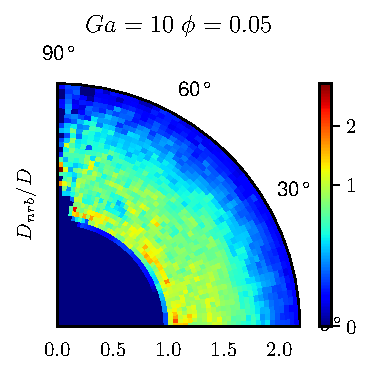
\includegraphics[width=4cm]{image/HOMOGENEOUS/fDrop/Pnst_mu_r_0_1_Ga_10_PHI_0_05}
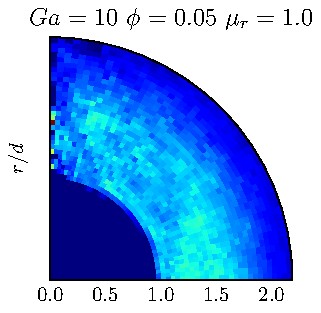
\includegraphics[width=4cm]{image/HOMOGENEOUS/fDrop/Pnst_mu_r_1_0_Ga_10_PHI_0_05}
\end{figure}

\JL{a on la meme echelle de couleur entre les deux graphiques, les cas Ga=5 ne semblent pas converger ? a virer ...}

Pas de position preferentiel dans ce cas

\paragraph{high $\phi$}
\begin{figure}
\centering
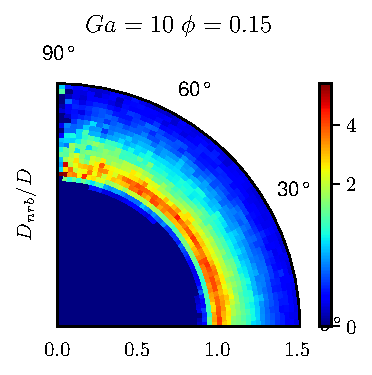
\includegraphics[width=4cm]{image/HOMOGENEOUS/fDrop/Pnst_mu_r_0_1_Ga_10_PHI_0_15}
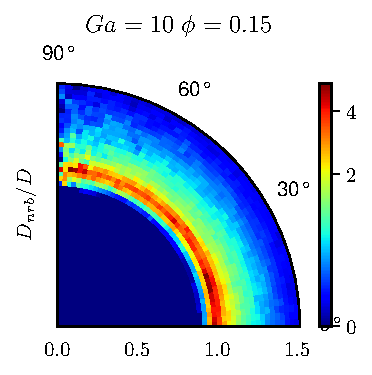
\includegraphics[width=4cm]{image/HOMOGENEOUS/fDrop/Pnst_mu_r_1_0_Ga_10_PHI_0_15}
\end{figure}

Idem pas de position preferentiel a discuter a la lumiere de la litterature (qui tends a dire le contraire ?). En regime de Stokes pas d'effet significatif du rapport de viscosité sur les pertubations. 







\subsubsection{Map at high $Ar$}

\paragraph{low $\phi$}
\begin{figure}
\centering
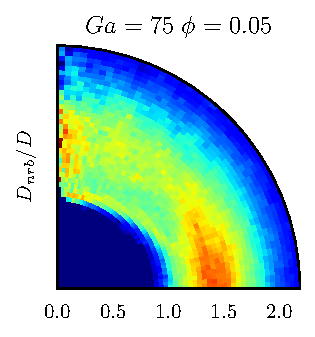
\includegraphics[width=4cm]{image/HOMOGENEOUS/fDrop/Pnst_mu_r_0_1_Ga_75_PHI_0_05}
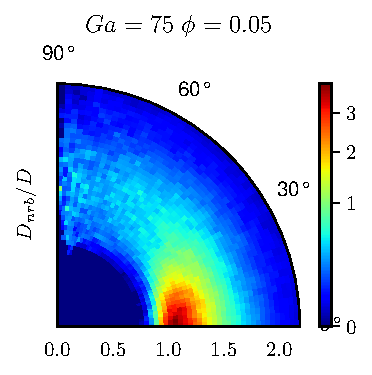
\includegraphics[width=4cm]{image/HOMOGENEOUS/fDrop/Pnst_mu_r_1_0_Ga_75_PHI_0_05}
\end{figure}

enorme effet du rapport de viscosité (donc a priori du sillage).
\JL{il manque des cas a Ga=100 ?}


\paragraph{high $\phi$}
\begin{figure}
\centering
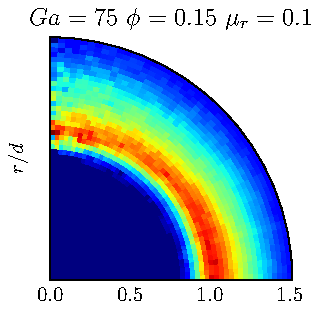
\includegraphics[width=4cm]{image/HOMOGENEOUS/fDrop/Pnst_mu_r_0_1_Ga_75_PHI_0_15}
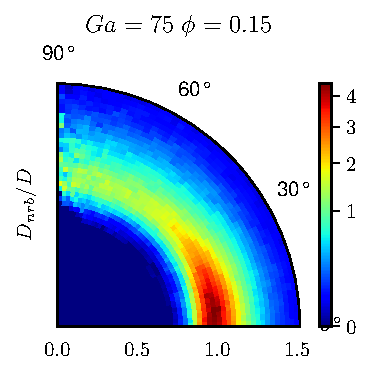
\includegraphics[width=4cm]{image/HOMOGENEOUS/fDrop/Pnst_mu_r_1_0_Ga_75_PHI_0_15}
\end{figure}

\subsubsection{...}


\begin{figure}
    \centering
    \begin{tikzpicture}
        \node at (0,0){ 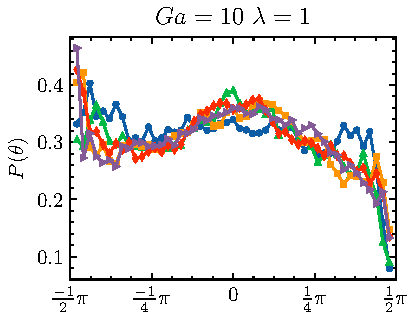
\includegraphics[height=0.3\textwidth]{image/HOMOGENEOUS/fDrop/Pnst_theta_mu_r_1_0_Ga_10.pdf} };
        \node at (0.4\textwidth,0){ 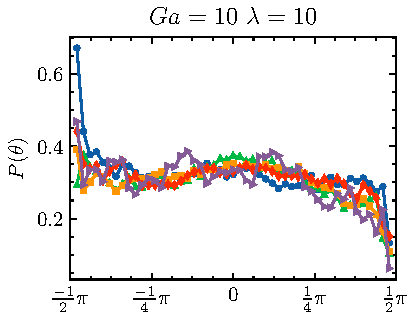
\includegraphics[height=0.3\textwidth]{image/HOMOGENEOUS/fDrop/Pnst_theta_mu_r_0_1_Ga_10.pdf} };
        \node at (0,-0.3\textwidth){ 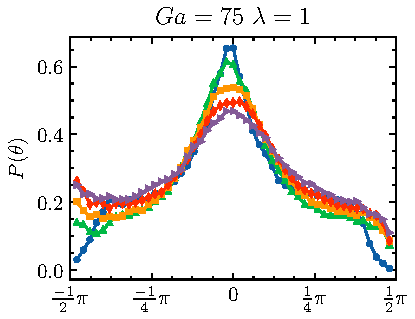
\includegraphics[height=0.3\textwidth]{image/HOMOGENEOUS/fDrop/Pnst_theta_mu_r_1_0_Ga_75.pdf} };
        \node at (0.4\textwidth,-0.3\textwidth){ 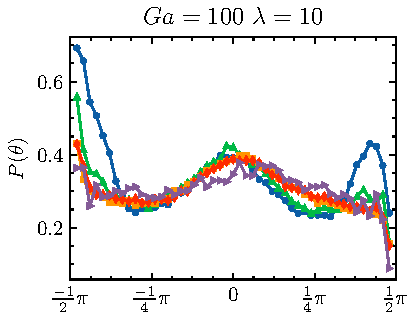
\includegraphics[height=0.3\textwidth]{image/HOMOGENEOUS/fDrop/Pnst_theta_mu_r_0_1_Ga_100.pdf} };
        % \node at (0,-0.6\textwidth){ 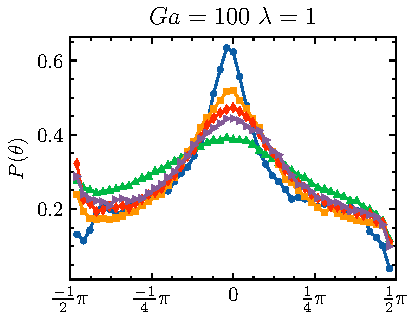
\includegraphics[height=0.3\textwidth]{image/HOMOGENEOUS/fDrop/Pnst_theta_mu_r_1_0_Ga_100.pdf} };
        % \node at (0.4\textwidth,-0.6\textwidth){ 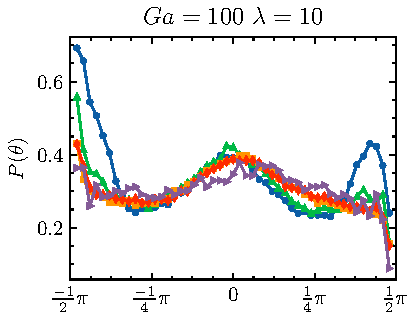
\includegraphics[height=0.3\textwidth]{image/HOMOGENEOUS/fDrop/Pnst_theta_mu_r_0_1_Ga_100.pdf} };
    \end{tikzpicture}
    \caption{Probability density function of the nearest particles : $P_{nst}(\theta)$ for different $Ga$ and $\lambda$. 
    Increasing $Ga$ from top to bottom, (left) $\lambda = 1$ (right) $\lambda = 10$. 
    The symbols correspond to different volume fraction ($\bullet$) $\phi = 1\%$, ($\blacktriangle$) $\phi = 5\%$, ($\blacksquare$) $\phi = 10\%$, ($\blacklozenge$) $\phi = 15\%$ and ($\blacktriangleright$) $\phi = 20\%$.
    (dashed lines) empirical formulas }
    \label{fig:P_nst_theta}
\end{figure}
By using polar coordinate such that $d \textbf{r} = r^2 \sin \phi dr d\phi d\theta$ we can further reduce the PDF to the only consideration of the angular dependency $\theta$ or the distance dependency $r$. 
These reduced p.d.f can be computed as follow, 
\begin{align*}
    P_{nst}(r) 
    &= \int_{-\pi/2}^{\pi/2}\int_{0}^{2\theta} P_{nst}(\textbf{x},\textbf{r},t) \sin \theta  d\phi d\theta\\
    P_{nst}(\theta)
    &= \int_{0}^{\infty}\int_{0}^{2\theta} P_{nst}(\textbf{x},\textbf{r},t) r^2  dr d\phi
\end{align*}
\tb{Check if those formulas are true}
Then $P_{nst}(\theta)$ is the probability that the nearest neighbor of a test particle is inclined at an angle $\theta$ relative to the flow direction. 
We observe that the particles pair becomes oriented with increasing $Ga$ and decreasing volume fraction

On \ref{fig:P_nst_theta} we observe that the particles pair becomes oriented with increasing $Ga$ and decreasing volume fraction.
Indeed, we observe a clear peak of $P_{nst}(\theta)$ at $\theta = \frac{\pi}{2}$. 
It seems that this tendency was also reported for spherical bubble in air-water system \citet{bunner2003effect}. 
Additionally, from \ref{fig:P_nst_theta} we can say that the viscosity ratio $\lambda$ seem to prevent the alignment/clustering of particles denoted by the slightly low peak for $\lambda =10$. 
\tb{Compart the Orientation with bubbly and solid flows \citet{roghair2011drag}}

\begin{figure}
    \centering
    \begin{tikzpicture}
        \node at (0,0){ 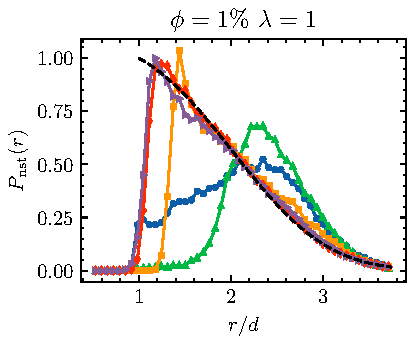
\includegraphics[height=0.3\textwidth]{image/HOMOGENEOUS/fDrop/Pnst_r_mu_r_1_0_PHI_1.pdf} };
        \node at (0.4\textwidth,0){ 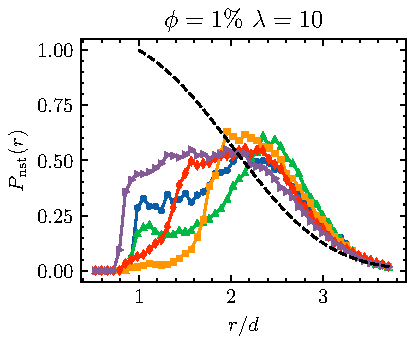
\includegraphics[height=0.3\textwidth]{image/HOMOGENEOUS/fDrop/Pnst_r_mu_r_0_1_PHI_1.pdf} };
        \node at (0,-0.3\textwidth){ 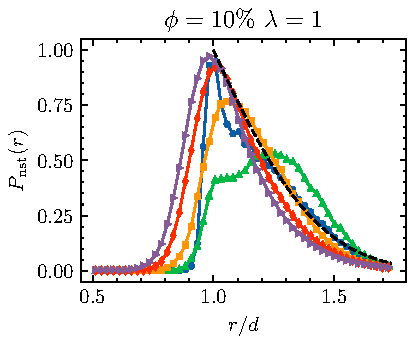
\includegraphics[height=0.3\textwidth]{image/HOMOGENEOUS/fDrop/Pnst_r_mu_r_1_0_PHI_10.pdf} };
        \node at (0.4\textwidth,-0.3\textwidth){ 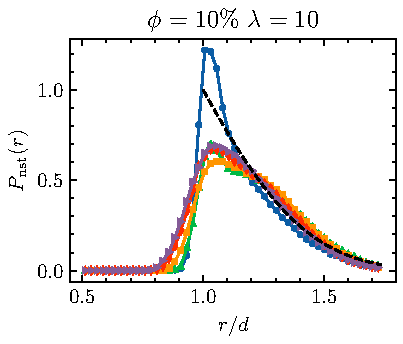
\includegraphics[height=0.3\textwidth]{image/HOMOGENEOUS/fDrop/Pnst_r_mu_r_0_1_PHI_10.pdf} };
        \node at (0,-0.6\textwidth){ 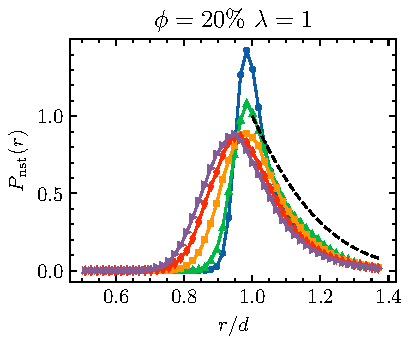
\includegraphics[height=0.3\textwidth]{image/HOMOGENEOUS/fDrop/Pnst_r_mu_r_1_0_PHI_20.pdf} };
        \node at (0.4\textwidth,-0.6\textwidth){ 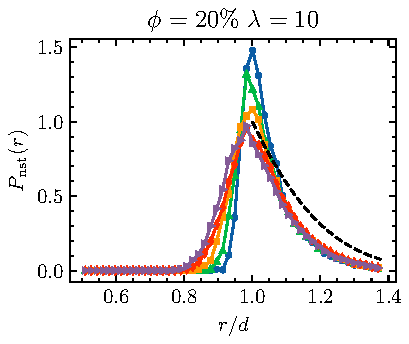
\includegraphics[height=0.3\textwidth]{image/HOMOGENEOUS/fDrop/Pnst_r_mu_r_0_1_PHI_20.pdf} };
    \end{tikzpicture}
    \caption{Radial probability density function : $P_{nst}(r)$ for different $\phi$ and $\lambda$. 
    Increasing $\phi$ from top to bottom, (left) $\lambda = 1$ (right) $\lambda = 10$. 
    The symbols correspond to different Galileo number ($\bullet$) $Ga = 10$, ($\blacktriangle$) $Ga = 25$, ($\blacksquare$) $Ga = 50$, ($\blacklozenge$) $Ga = 75$ and ($\blacktriangleright$) $Ga = 100$.
    (dashed lines) Theoretical formula \ref{eq:P_nst_r}}
    \label{fig:P_nst_r}
\end{figure}
Note that for solid spherical particle in the dilute regime a theoretical formula for $P_{nst}(r)$ can be found assuming completely random distribution and no interactions nor overlap between particles \citep{zhang2021ensemble}, it reads, 
\begin{equation*}
    P_\text{nst}^\text{th}(r) = n_p e^{-4 \pi n_p (r^3 - d^3)/3}.
    \label{eq:P_nst_r}
\end{equation*}
It is evident that all the distribution presented \ref{fig:P_nst_r} have a peak at $r > 1$ where the theoretical formula  predict a peak at $r=1$. 
This is obviously due to the fact that we are in presence of particles interaction which tends to repulse the particles from each others and therefore to shift the distribution to the left. 
What is more interesting is that for $\lambda = 1$ at low volume fraction and high \textit{Galileo} we are able to recover approximately the random particle distribution $P_\text{nst}^\text{th}$ with our numerical results. 
Whereas for $\lambda = 10$ the particle are relatively maintained far from  each other as depicted \ref{fig:P_nst_r}(right). 
We can stipulate that for high viscosity ratio the particles have a tendency to generate more particle fluid mediated interaction as demonstrated by the flow lines \ref{fig:Stream}.


\subsection{Nearest-particle average fluid velocity}
Objectives : 
\begin{itemize}
    \item Problematic "How to analyse the flow around a particle in average"
    \item First : present the averaged the nearest particles' statistics method. And how to compute the nearest averaged velocity fields $\nstavg{\textbf{u}}$.
    \item Present the flowlines and show that for $\phi = 5 \rightarrow 20\%$ we observe that a vertical symmetry arise.
    \item Explain how this field it is related to the velocity fluctuation with \ref{eq:def_uu}
    \item Conclude that these velocity fields represent the PWFs since it represent the mean wakes \citep{du2022analysis}.  
    \item Additionally, some comment can be made regarding the shape of the particle thanks to the contour lines. 
    \item Approach these flow fields by analytical solution of potential flow to obtain an analytical solution for teh reyolds stress. 
\end{itemize}

Presently, we wish to investigate the  averaged flow structure around a fluid particle.
To obtain such a field we make use of the nearest particle statistics recently introduced by \citet{zhang2021stress}. 
We introduce $\nstavg{\textbf{u}}(\textbf{x},\textbf{r})$ as the velocity fields at \textbf{x} knowing there is a particles center of mass located at \textbf{r}.
Additionally, this particle is the nearest particle among all to the point \textbf{x}.  
Formally, this conditional average can be written as, 
\begin{equation}
    \nstavg{\textbf{u}}(\textbf{x},\textbf{r})=\frac{1}{P_{nst}(\textbf{x},\textbf{r})} 
    \int \textbf{u}(\textbf{x},\CC,t) 
    \sum_{\alpha}\delta(\textbf{x}+\textbf{r}-\textbf{x}^\alpha(\CC,t)) h_{\alpha}(\CC,\textbf{x},t) d\mathscr{P} 
    \label{eq:q_nst_avg}
\end{equation}
where $P_{nst}(\textbf{x},\textbf{r})$ is defined as,  
\begin{equation}
    P_{nst}(\textbf{x},\textbf{r})= 
    \int
    \sum_{\alpha}\delta(\textbf{x}+\textbf{r}-\textbf{x}^\alpha(\CC,t)) 
    h_\alpha(\CC,\textbf{x},t) d\mathscr{P}. 
    \label{eq:P_nsti}
\end{equation}
which is the probability of finding a particle center of mass at a distance \textbf{r} from the point \textbf{x} knowing that this particle is the nearest neighbor to the points \textbf{x}. 
The function $h_\alpha$ is defined such that, $h_\alpha = 1/N^p$ if $\alpha$ is the nearest particle to \textbf{x} and $0$ if not, where $N^p$ is the total number of nearest neighbor.
Indeed, the point \textbf{x} at mid-distance from two particles posses two nearest neighbors by definition, thus $N(\textbf{x},\CC,t) = 2$ in this case. 

\tb{Include the numerical computaiton of $\nstavg{\textbf{u}}$.  }

\ref{fig:Stream} shows the streamline of the field $\nstavg{\textbf{u}}(\textbf{x},\textbf{r})$ for three volume fractions. 
We clearly observe the induced wake of the particles centered at the origin. 

\begin{figure}[h!]
    \centering
    \begin{tikzpicture}
        \node (img) at (0,0)  {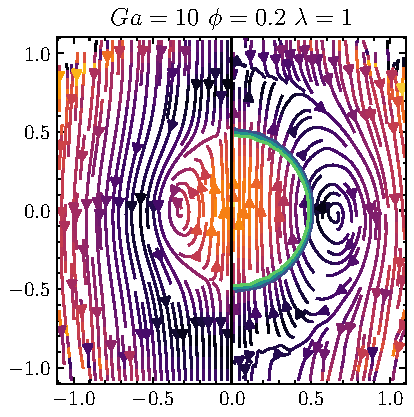
\includegraphics[height=0.3\textwidth]{image/HOMOGENEOUS/Stream/Stream_PHI_20_Ga_10_l_1.pdf}};
        \node (img) at (0.3\textwidth,0)  {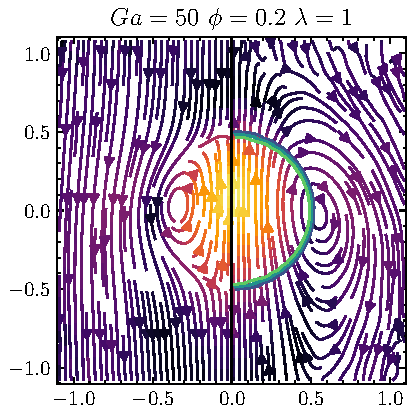
\includegraphics[height=0.3\textwidth]{image/HOMOGENEOUS/Stream/Stream_PHI_20_Ga_50_l_1.pdf}};
        \node (img) at (0.6\textwidth,0)  {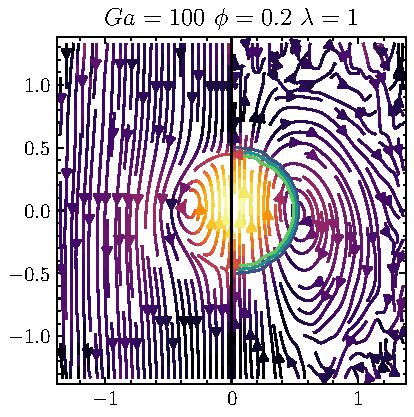
\includegraphics[height=0.3\textwidth]{image/HOMOGENEOUS/Stream/Stream_PHI_20_Ga_100_l_1.pdf}};
        \node (img) at (0,-0.3\textwidth)  {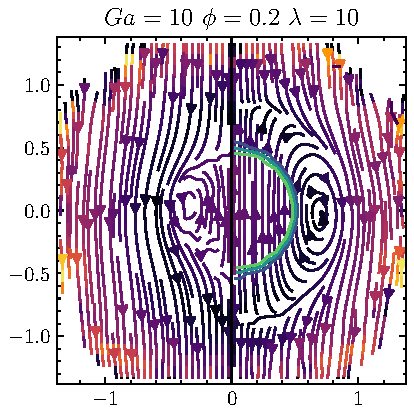
\includegraphics[height=0.3\textwidth]{image/HOMOGENEOUS/Stream/Stream_PHI_20_Ga_10_l_10.pdf}};
        \node (img) at (0.3\textwidth,-0.3\textwidth)  {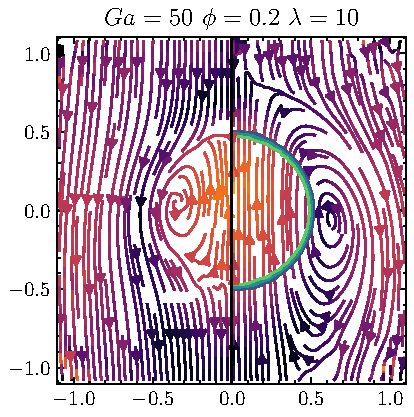
\includegraphics[height=0.3\textwidth]{image/HOMOGENEOUS/Stream/Stream_PHI_20_Ga_50_l_10.pdf}};
        \node (img) at (0.6\textwidth,-0.3\textwidth)  {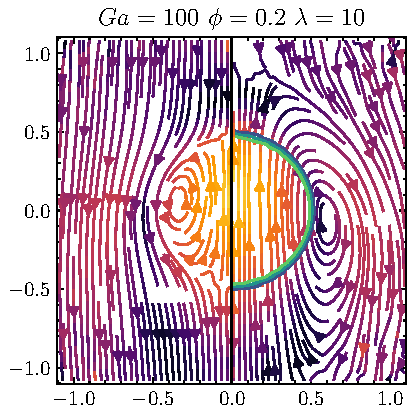
\includegraphics[height=0.3\textwidth]{image/HOMOGENEOUS/Stream/Stream_PHI_20_Ga_100_l_10.pdf}};
        \node (img) at (0,-0.6\textwidth)  {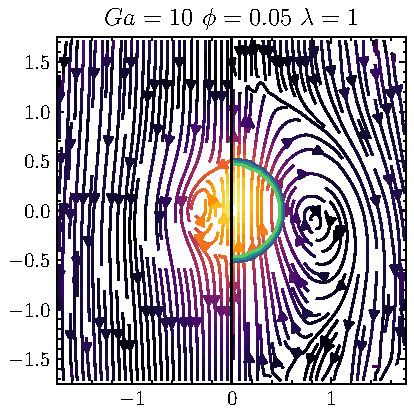
\includegraphics[height=0.3\textwidth]{image/HOMOGENEOUS/Stream/Stream_PHI_5_Ga_10_l_1.pdf}};
        \node (img) at (0.3\textwidth,-0.6\textwidth)  {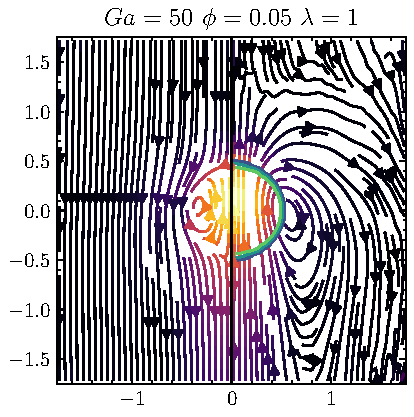
\includegraphics[height=0.3\textwidth]{image/HOMOGENEOUS/Stream/Stream_PHI_5_Ga_50_l_1.pdf}};
        \node (img) at (0.6\textwidth,-0.6\textwidth)  {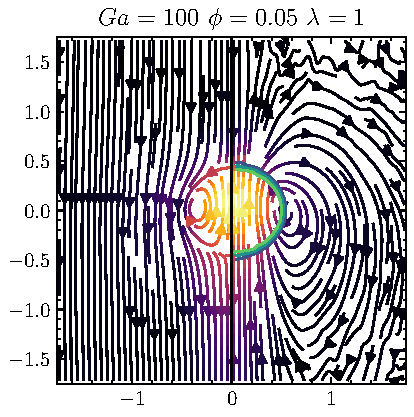
\includegraphics[height=0.3\textwidth]{image/HOMOGENEOUS/Stream/Stream_PHI_5_Ga_100_l_1.pdf}};
        \node (img) at (0,-0.9\textwidth)  {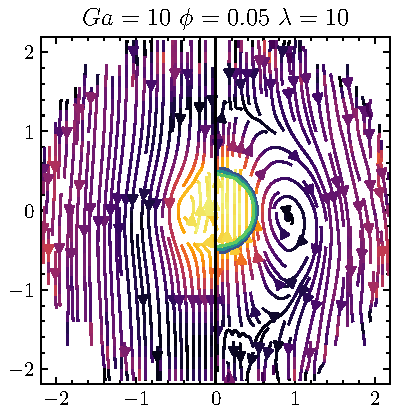
\includegraphics[height=0.3\textwidth]{image/HOMOGENEOUS/Stream/Stream_PHI_5_Ga_10_l_10.pdf}};
        \node (img) at (0.3\textwidth,-0.9\textwidth)  {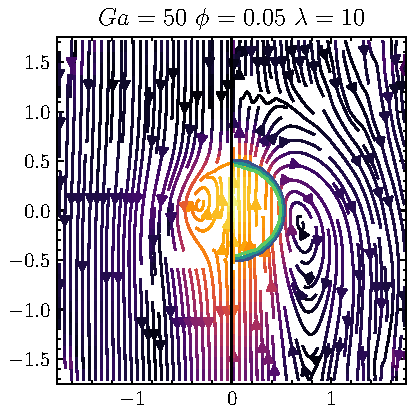
\includegraphics[height=0.3\textwidth]{image/HOMOGENEOUS/Stream/Stream_PHI_5_Ga_50_l_10.pdf}};
        \node (img) at (0.6\textwidth,-0.9\textwidth)  {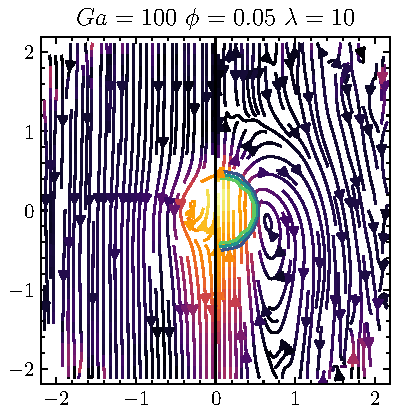
\includegraphics[height=0.3\textwidth]{image/HOMOGENEOUS/Stream/Stream_PHI_5_Ga_100_l_10.pdf}};
    \end{tikzpicture}
    \caption{Nearest particle averaged velocity $\nstavg{\textbf{u}}(\textbf{r})$ for  $\phi = 5\%$ and $20\%$.
    Green lines : contour plots of the nearest averaged indicator function $\nstavg{\chi_d}(\textbf{r})$ (it represent the mean shape of the particles)}
    \label{fig:Stream}
\end{figure}
% \begin{figure}[h!]
%     \centering
%     \begin{tikzpicture}
%         \node (img) at (0,0)  {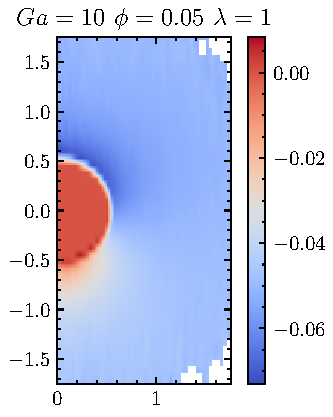
\includegraphics[height=0.4\textwidth]{image/HOMOGENEOUS/Stream/P_PHI_5_Ga_10_l_1.pdf}};
%         \node (img) at (0.3\textwidth,0)  {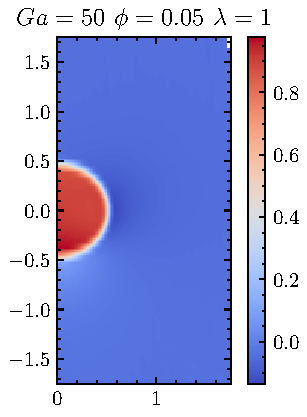
\includegraphics[height=0.4\textwidth]{image/HOMOGENEOUS/Stream/P_PHI_5_Ga_50_l_1.pdf}};
%         \node (img) at (0.6\textwidth,0)  {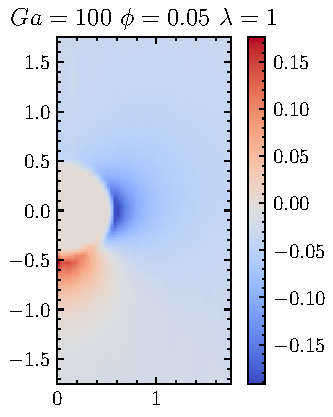
\includegraphics[height=0.4\textwidth]{image/HOMOGENEOUS/Stream/P_PHI_5_Ga_100_l_1.pdf}};
%         \node (img) at (0,0.4\textwidth)  {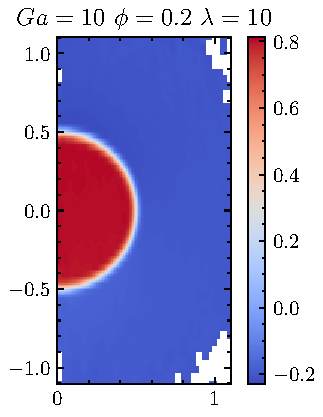
\includegraphics[height=0.4\textwidth]{image/HOMOGENEOUS/Stream/P_PHI_20_Ga_10_l_10.pdf}};
%         \node (img) at (0.3\textwidth,0.4\textwidth)  {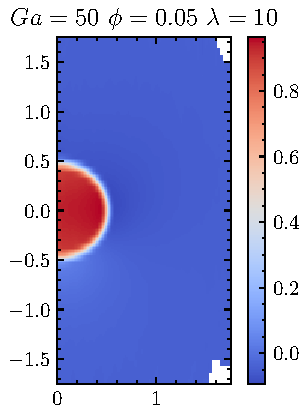
\includegraphics[height=0.4\textwidth]{image/HOMOGENEOUS/Stream/P_PHI_5_Ga_50_l_10.pdf}};
%         \node (img) at (0.6\textwidth,0.4\textwidth)  {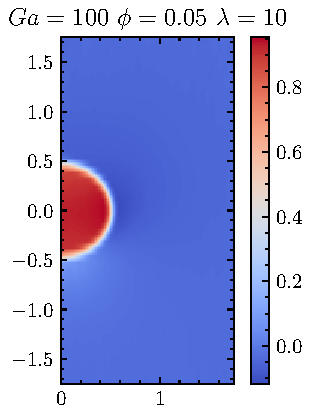
\includegraphics[height=0.4\textwidth]{image/HOMOGENEOUS/Stream/P_PHI_5_Ga_100_l_10.pdf}};
%     \end{tikzpicture}
%     \caption{Nearest particle averaged pressure $\nstavg{p}(\textbf{r})$ normalized by the Laplace pressure $4 \gamma /d$ for  $\phi = 5\%$ and $20\%$}
%     \label{fig:Stream}
% \end{figure}
\begin{figure}[h!]
    \centering
    \begin{tikzpicture}
        \node (img) at (0,0)  {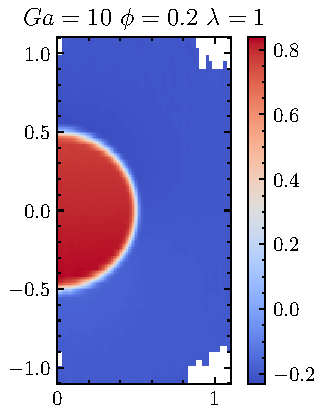
\includegraphics[height=0.3\textwidth]{image/HOMOGENEOUS/Stream/P_PHI_20_Ga_10_l_1.pdf}};
        \node (img) at (0.3\textwidth,0)  {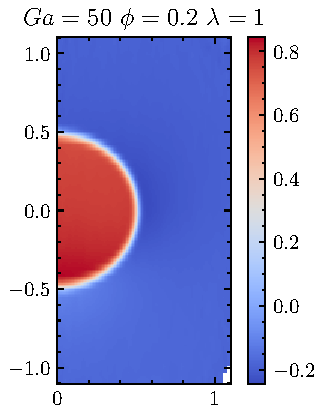
\includegraphics[height=0.3\textwidth]{image/HOMOGENEOUS/Stream/P_PHI_20_Ga_50_l_1.pdf}};
        \node (img) at (0.6\textwidth,0)  {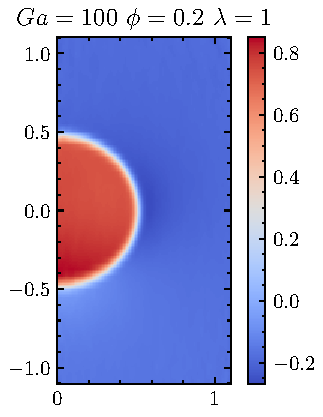
\includegraphics[height=0.3\textwidth]{image/HOMOGENEOUS/Stream/P_PHI_20_Ga_100_l_1.pdf}};
        \node (img) at (0,-0.3\textwidth)  {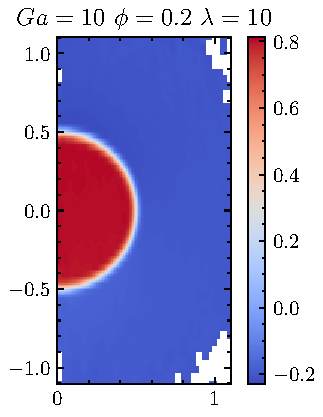
\includegraphics[height=0.3\textwidth]{image/HOMOGENEOUS/Stream/P_PHI_20_Ga_10_l_10.pdf}};
        \node (img) at (0.3\textwidth,-0.3\textwidth)  {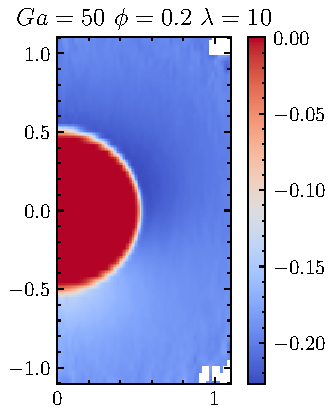
\includegraphics[height=0.3\textwidth]{image/HOMOGENEOUS/Stream/P_PHI_20_Ga_50_l_10.pdf}};
        \node (img) at (0.6\textwidth,-0.3\textwidth)  {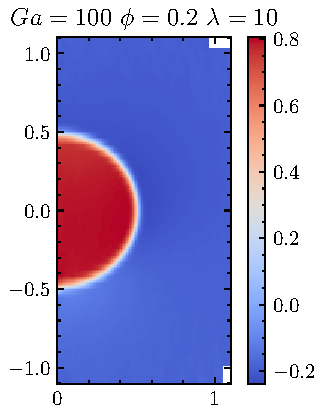
\includegraphics[height=0.3\textwidth]{image/HOMOGENEOUS/Stream/P_PHI_20_Ga_100_l_10.pdf}};
        \node (img) at (0,-0.6\textwidth)  {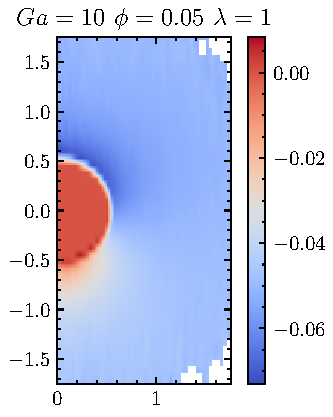
\includegraphics[height=0.3\textwidth]{image/HOMOGENEOUS/Stream/P_PHI_5_Ga_10_l_1.pdf}};
        \node (img) at (0.3\textwidth,-0.6\textwidth)  {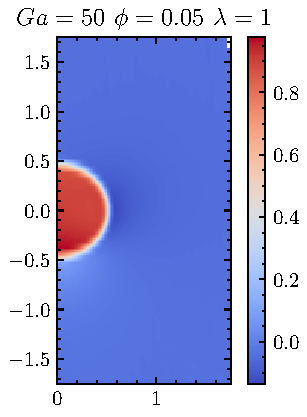
\includegraphics[height=0.3\textwidth]{image/HOMOGENEOUS/Stream/P_PHI_5_Ga_50_l_1.pdf}};
        \node (img) at (0.6\textwidth,-0.6\textwidth)  {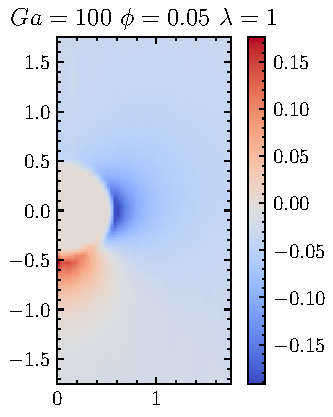
\includegraphics[height=0.3\textwidth]{image/HOMOGENEOUS/Stream/P_PHI_5_Ga_100_l_1.pdf}};
        % \node (img) at (0,-0.9\textwidth)  {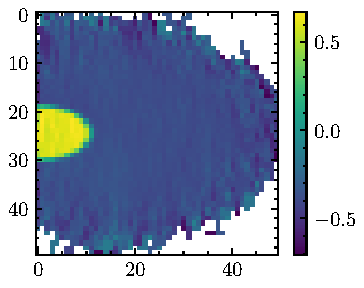
\includegraphics[height=0.3\textwidth]{image/HOMOGENEOUS/Stream/P_PHI_5_Ga_10_l_10.pdf}};
        \node (img) at (0.3\textwidth,-0.9\textwidth)  {\includegraphics[height=0.3\textwidth]{image/HOMOGENEOUS/Stream/P_PHI_5_Ga_50_l_10.pdf}};
        \node (img) at (0.6\textwidth,-0.9\textwidth)  {\includegraphics[height=0.3\textwidth]{image/HOMOGENEOUS/Stream/P_PHI_5_Ga_100_l_10.pdf}};
    \end{tikzpicture}
    \caption{Nearest particle averaged pressure $\nstavg{p}(\textbf{r})$ normalized by the Laplace pressure $4 \gamma /d$ for  $\phi = 5\%$ and $20\%$}  
    \label{fig:Stream}
\end{figure}
It is evident from these plots that the induced wake is the averaged wake resulting from the averaged translation of the particles. 
And this averaged wake has a tendency to be asymmetrical for low volume fraction and symmetrical for higher ones. 
Additionally, form basic mathematical consideration on the average operators we can demonstrate that :
\begin{multline*}
    \avg{\chi_k \textbf{u}'_k\textbf{u}'_k}(\textbf{x},t)
    + \phi_k \textbf{u}_k\textbf{u}_k
    = \\
    \underbrace{\int (\nstavg{\chi_k \textbf{u}^0_k}  \nstavg{\chi_k \textbf{u}^0_k} / (\nstavg{\chi_k})  P_{nst}(\textbf{x},t,\textbf{r}) d\textbf{r} }_\text{PWFs}
    +\underbrace{\int \nstavg{\chi_k \textbf{v}_k^0\textbf{v}_k^0}  P_{nst}(\textbf{x},t,\textbf{r}) d\textbf{r}}_\text{WIA}
    \label{eq:def_uu}
\end{multline*}
where, $\textbf{v}_k^0  = \textbf{u}_k^0 - \nstavg{\chi_k \textbf{u}^0_k} / \nstavg{\chi_k}$ is the fluctuation of the local velocity relative to the nearest averaged value. 
Consequently, we can decompose the ensemble averaged fluid velocity fluctuations with a first term representing the variance of $\nstavg{\textbf{u}}$ around the mean $\textbf{u}_k$, and a second term representing the variance of $\textbf{u}^0_k$ around the mean  $\nstavg{\textbf{u}}$. 

There are two phenomena causing velocity fluctuations in the liquid:
the agitation resulting from wakes and their collective interactions [wake-induced agitation (WIA)], and the non-turbulent fluctuations resulting from averaged wakes and potential flows around bubbles [potential flow and averaged wake fluctuations (PWFs)].
As a matter of fact in the phase space of $\nstavg{\textbf{u}}(\textbf{r})$ the bubble is fixed at the origin thus we recover the velocity fields representing what is called the PWFs. 
In their study \citet{du2022analysis} carry out transient simulation with fixed particles to recover the PWFs components here we show that a single simulation permit us to recover WIA and PWFs by the mean of the nearest particles' statistics. 

\tb{make the link with drag force/drag coef  \citet{dandy1989buoyancy}}
\tb{make the link with velocity fluctuation \citet{almeras2021statistics}}





\subsection{Nearest averaged particle center of mass velocity}
\subsubsection{Nearest averaged particle center of mass velocity in the dispersed phase reference frame}
\begin{equation}
    \nstavg{\textbf{u}^i}=\frac{1}{P_{nst}(\textbf{x},\textbf{r},t)} 
    \int \sum_{i}\delta(\textbf{x}-\textbf{x}^i(\CC,t))
    \sum_{j\neq i}\delta(\textbf{x}+\textbf{r}-\textbf{x}^j(\CC,t)) 
    % \delta(t+a-t_c^{ij}(\CC,t)) 
    h_{ij}(\CC,t) 
    \textbf{u}^i(\CC,t)
    d\mathscr{P} 
    - \textbf{u}_p
\end{equation}
\subsubsection{Nearest averaged particle center of mass relative velocity}
\begin{equation}
    \nstavg{\textbf{w}}=\frac{1}{P_{nst}(\textbf{x},\textbf{r},t)} 
    \int \sum_{i}\delta(\textbf{x}-\textbf{x}^i(\CC,t))
    \sum_{j\neq i}\delta(\textbf{x}+\textbf{r}-\textbf{x}^j(\CC,t)) 
    % \delta(t+a-t_c^{ij}(\CC,t)) 
    h_{ij}(\CC,t) 
    (\textbf{u}^i(\CC,t) - \textbf{u}^j(\CC,t))
    d\mathscr{P} 
\end{equation}


\begin{figure}[h!]
    \centering
    \begin{tikzpicture}
        \node (img) at (0,0)  {\includegraphics[height=0.3\textwidth]{image/HOMOGENEOUS/fDrop/U_l_1_Ga_10_PHI_20.pdf}};
        \node (img) at (0.3\textwidth,0)  {\includegraphics[height=0.3\textwidth]{image/HOMOGENEOUS/fDrop/U_l_1_Ga_50_PHI_20.pdf}};
        \node (img) at (0.6\textwidth,0)  {\includegraphics[height=0.3\textwidth]{image/HOMOGENEOUS/fDrop/U_l_1_Ga_100_PHI_20.pdf}};
        \node (img) at (0,-0.3\textwidth)  {\includegraphics[height=0.3\textwidth]{image/HOMOGENEOUS/fDrop/U_l_10_Ga_10_PHI_20.pdf}};
        \node (img) at (0.3\textwidth,-0.3\textwidth)  {\includegraphics[height=0.3\textwidth]{image/HOMOGENEOUS/fDrop/U_l_10_Ga_50_PHI_20.pdf}};
        \node (img) at (0.6\textwidth,-0.3\textwidth)  {\includegraphics[height=0.3\textwidth]{image/HOMOGENEOUS/fDrop/U_l_10_Ga_100_PHI_20.pdf}};
        \node (img) at (0,-0.6\textwidth)  {\includegraphics[height=0.3\textwidth]{image/HOMOGENEOUS/fDrop/U_l_1_Ga_10_PHI_5.pdf}};
        \node (img) at (0.3\textwidth,-0.6\textwidth)  {\includegraphics[height=0.3\textwidth]{image/HOMOGENEOUS/fDrop/U_l_1_Ga_50_PHI_5.pdf}};
        \node (img) at (0.6\textwidth,-0.6\textwidth)  {\includegraphics[height=0.3\textwidth]{image/HOMOGENEOUS/fDrop/U_l_1_Ga_75_PHI_5.pdf}};
        \node (img) at (0,-0.9\textwidth)  {\includegraphics[height=0.3\textwidth]{image/HOMOGENEOUS/fDrop/U_l_10_Ga_10_PHI_5.pdf}};
        \node (img) at (0.3\textwidth,-0.9\textwidth)  {\includegraphics[height=0.3\textwidth]{image/HOMOGENEOUS/fDrop/U_l_10_Ga_50_PHI_5.pdf}};
        \node (img) at (0.6\textwidth,-0.9\textwidth)  {\includegraphics[height=0.3\textwidth]{image/HOMOGENEOUS/fDrop/U_l_10_Ga_75_PHI_5.pdf}};
    \end{tikzpicture}
    \caption{Nearest particle averaged pressure velocity $\nstavg{\textbf{u}^i}(\textbf{r}) - \textbf{u}_p$ }  
    \ref{fig:u_nst}
\end{figure}
% \begin{figure}[h!]
%     \centering
%     \begin{tikzpicture}
%         \node (img) at (0,0)  {\includegraphics[height=0.3\textwidth]{image/HOMOGENEOUS/fDrop/U_rel_l_1_Ga_10_PHI_20.pdf}};
%         \node (img) at (0.3\textwidth,0)  {\includegraphics[height=0.3\textwidth]{image/HOMOGENEOUS/fDrop/U_rel_l_1_Ga_50_PHI_20.pdf}};
%         \node (img) at (0.6\textwidth,0)  {\includegraphics[height=0.3\textwidth]{image/HOMOGENEOUS/fDrop/U_rel_l_1_Ga_100_PHI_20.pdf}};
%         \node (img) at (0,-0.3\textwidth)  {\includegraphics[height=0.3\textwidth]{image/HOMOGENEOUS/fDrop/U_rel_l_10_Ga_10_PHI_20.pdf}};
%         \node (img) at (0.3\textwidth,-0.3\textwidth)  {\includegraphics[height=0.3\textwidth]{image/HOMOGENEOUS/fDrop/U_rel_l_10_Ga_50_PHI_20.pdf}};
%         \node (img) at (0.6\textwidth,-0.3\textwidth)  {\includegraphics[height=0.3\textwidth]{image/HOMOGENEOUS/fDrop/U_rel_l_10_Ga_100_PHI_20.pdf}};
%         \node (img) at (0,-0.6\textwidth)  {\includegraphics[height=0.3\textwidth]{image/HOMOGENEOUS/fDrop/U_rel_l_1_Ga_10_PHI_5.pdf}};
%         \node (img) at (0.3\textwidth,-0.6\textwidth)  {\includegraphics[height=0.3\textwidth]{image/HOMOGENEOUS/fDrop/U_rel_l_1_Ga_50_PHI_5.pdf}};
%         \node (img) at (0.6\textwidth,-0.6\textwidth)  {\includegraphics[height=0.3\textwidth]{image/HOMOGENEOUS/fDrop/U_rel_l_1_Ga_75_PHI_5.pdf}};
%         \node (img) at (0,-0.9\textwidth)  {\includegraphics[height=0.3\textwidth]{image/HOMOGENEOUS/fDrop/U_rel_l_10_Ga_10_PHI_5.pdf}};
%         \node (img) at (0.3\textwidth,-0.9\textwidth)  {\includegraphics[height=0.3\textwidth]{image/HOMOGENEOUS/fDrop/U_rel_l_10_Ga_50_PHI_5.pdf}};
%         \node (img) at (0.6\textwidth,-0.9\textwidth)  {\includegraphics[height=0.3\textwidth]{image/HOMOGENEOUS/fDrop/U_rel_l_10_Ga_75_PHI_5.pdf}};
%     \end{tikzpicture}
%     \caption{Nearest particle averaged pressure velocity $\nstavg{\textbf{w}}(\textbf{r})$ }  
%     \ref{fig:w_nst}
% \end{figure}


\section{Conclusion}
\section{Conclusion}

% \citet{einstein1905neue,taylor1932viscosity} demonstrated how the first moment of the hydrodynamic forces (Stresslet) applied on a particle immersed in pure linear flow induced an additional viscosity to the mixture. 
% Later~\citet{zhang1994ensemble,lhuillier1996contribution,jackson1997locally,zhang1997momentum} demonstrated that the second moment of forces were also contributing to the stresses inducing a non-newtonian behaviors, even in the Stokes and dilute limit.  

In this work we computed the moments of force on the surface of a test droplet in the situation of uniform relative motions between the droplet and the continuous phase. 
We considered low but finite Reynolds number $Re$. 
The averaged first moment of force is given by~\ref{eq:forces_reformulated2_avg}, scales as $O(\rho_f \phi u_r^2)$, hence contributing to the averaged Stress of the suspension on the same ground as  \citet{einstein1905neue} or \citep{taylor1932viscosity} correction to the viscosity of the mixture. 
In a lesser extend the inertial part of the second moment also contribute to the Rheology. 
This first point constitutes the main result of the paper. 

Others important conclusion reached through this work includes: a general reciprocal formula to derive the forces and moments on droplets, and the explicit appearing of the velocity variance term in the drag force term. 







\appendix
%\section{Statistical convergence and mesh independence studies}
\section{Numerical validations}
\label{ap:A}
\subsection{Validation test cases}
The \texttt{Basilisk} code has been validated numerous time in previous numerical studies. 
Especially, we can cite the recent studies of \citet{innocenti2020direct} and \citet{hidman2023assessing} which both performed DNS of rising suspension of bubbles. 
Nevertheless, in this work we investigate specific statistical distribution,
and we make use of a multi-VoF method to avoid droplets coalescence, therefore a meticulous validation of the DNS is in order. 
We start by presenting a brief comparison with the reference DNS \citet{esmaeeli1999direct}. 
Afterward we present a study focusing on the interfaces' kinematic, we compare our DNS with the experimental results of \citet{mohamed2003drop} in the objective to show that the Multi-VoF method indeed capture the physics of two colliding interfaces without solving the flows in the film. 
Once the mesh and the physics are validated, a study on the convergence of the statistics is presented. 

\subsection*{Ordered array of buoyant bubbles}

From our knowledge, no simulations nor experimental results have been carried out for rising buoyant viscous drop. 
Therefore, instead we reproduced the ordered array simulation of \citet{esmaeeli1999direct} with \texttt{Basilisk} to validate the mesh definition of our DNS.  
It consists in a 3-D buoyant ordered rising array of bubbles. 
In our notation the flow parameters of the simulation reads, 
\begin{align*}
    \lambda = 10,
    && \zeta = 10,
    && Bo = 1.8,
    && Ga = 28.37,
    && \phi = 0.125.
\end{align*}
\begin{figure}[h!]
    \centering
    \includegraphics[height = 0.3\textwidth]{image/VALIDATION2.0/Loisy/Re.pdf}
    \caption{Time evolution of the Reynolds number based on the instentaneous volume averaged drift velocity, $Re(t) = \rho_fU d /\mu_f$, with $U(t) = |\textbf{u}_p - \textbf{u}_f|$ with $\phi = 0.1256$, $\zeta =\mu_r =10$ and $Ga = 29.9$.
    $\textbf{u}_p$ and $\textbf{u}_f$ are the particle and fluid phase volume averaged velocity at time $t$.}
    \label{fig:ordered_array}
\end{figure}
\ref{fig:ordered_array} display our numerical simulation against the original result of \citet{esmaeeli1999direct}.
We observe very good agreements between both studies for all mesh definition.
Additionally, we displayed the results of \citet{innocenti2020direct} for $d/\Delta = 20$ to point out a divergence with our results at the same mesh definition.  
Both our simulations and the one of \citet{innocenti2020direct} have been carried out with the  \texttt{Basilisk} code. 
The cause of this difference is in fact due to a different method of interpolation used for the viscosity coefficient $\mu$. 
We used an arithmetic mean, whereas \citet{innocenti2020direct} used a 
harmonic mean.
As a matter of fact in this regime the arithmetic mean, which will be used in this work, permit us to reach a faster convergence. 
Overall these results indicate that the criterion $d/\Delta = 30$ seems sufficient, which is consistent with the aforementioned studies.


\subsection*{Drop impact on a liquid-liquid interface}

In section, we investigate in more detail the physics behind the Multi-VoF method. 
We need to verify if we accurately capture the physics of the droplets interfaces despite the fact that we do not model accurately  the film between two droplets. 
Following \citet{balcazar2015multiple} we reproduced the experiment of drop impact on a liquid–liquid interface carried by \citet{mohamed2003drop} but with the \texttt{Basilisk} code. 
This experiment consist in letting a drop fall into a pool of the same fluid as the drop, all along the experiment the interfaces of the droplets and the pool are tracked. 
In our notation the dimensionless parameters of latter study reads, 
\begin{align*}
    Ga = 71.02 
    && Bo = 6.40
    && \lambda = 0.33
    && \zeta = 1.189
\end{align*}
Following \citet{mohamed2003drop} we defined the dimensionless time $t / t_i = t U_i(t) /d$ where $U_i(t)$ is droplet velocity at $t<0$ and where $t=0$ is the time of impact. 
Regarding the geometry of the problem we sketched in \ref{fig:schemeLong} a scheme of the initial position of the droplet in the computational domain.
Additionally, we displayed on \ref{fig:schemeLong} a snapshot of the numerical domain were we see the drop colliding the pool's interface.
Both, the drop and the pool does not merge since we use the Multi-VoF method, note that in the experiment the drop does not merge with the pool either.
This enables us to represent with DNS a physical situation where the interfaces do not coalesce, but where we use a grid definition of $d/\Delta = 30$ which is of course not sufficient to model the flow inside the film. 
\begin{figure}[h!]
    \centering
    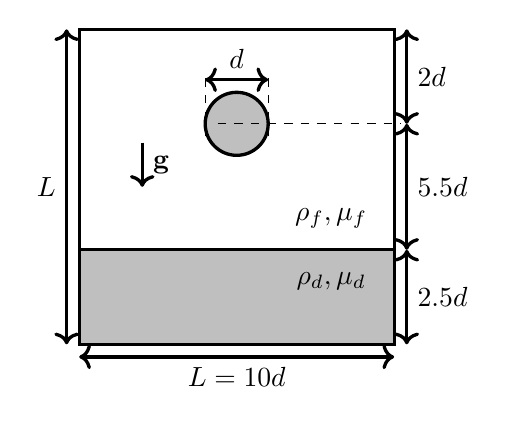
\begin{tikzpicture}[very thick,scale = 0.8]
        \draw (0,0) rectangle (5,5);
        \draw[fill=gray!50] (0,0) rectangle (5,1.5);
        \draw[fill=gray!50] (2.5,3.5) circle (0.5);
        \draw[<->](0,-0.2) --++ (5,0)node[midway,below]{$L  = 10 d$};
        \draw[<->](-0.2,0) --++ (0,5)node[midway,left]{$L$};
        \draw[<->](5.2,0) --++ (0,1.5)node[midway,right]{$2.5 d$};
        \draw[<->](5.2,1.5) --++ (0,2)node[midway,right]{$5.5 d$};
        \draw[<->](5.2,3.5) --++ (0,1.5)node[midway,right]{$ 2d$};
        \draw[dashed,thin](2.2,3.5) --++ (2.9,0);
        \draw[dashed,thin](2.2,3.5) --++ (2.9,0);
        \draw[->](1,3.2) --++ (0,-0.7)node[midway,right]{$\textbf{g}$};
        \draw[<->](2,4.2) --++ (1,0)node[midway,above]{$d$};
        \draw[thin,dashed](2,3.3) --++ (0,1);
        \draw[thin,dashed](3,3.3) --++ (0,1);
        \node (a) at (4,2){$\rho_f, \mu_f$};
        \node (a) at (4,1){$\rho_d, \mu_d$};
    \end{tikzpicture}
    \includegraphics[height = 0.3\textwidth]{image/VALIDATION2.0/Longmire/IMG/image-079.png}
    \caption{(left) Scheme of the computational set up at the initial time. 
    (right) Snapshot of the computational domain after the collision time, with the interfaces represented in gray.
    The background color represent the velocity field magnitude, which is undisturbed, indicating a large enough domain. }
    \label{fig:schemeLong}
\end{figure}
\begin{figure}[h!]
    \centering
    \includegraphics[height = 0.3\textwidth]{image/VALIDATION2.0/Longmire/Re.pdf}
    \includegraphics[height = 0.3\textwidth]{image/VALIDATION2.0/Longmire/Dist.pdf}
    \caption{(left) Time evolution of the Reynolds number based on the droplet velocity, $Re(t) = \rho_fU d /\mu_f$ in term of the dimensionless time, (+) numerical results of  \citet{balcazar2015multiple} (right)  position of the interfaces, ($\bullet$) top droplets surface, ($+$) bot droplet surface, (x) pool surface. (Symbols) experimental result of \citet{mohamed2003drop} (solid line) present numerical simulations with $d/\Delta = 30$. }
    \label{fig:resultslong}
\end{figure}
\ref{fig:resultslong} represent the comparison between our results against the experiment of \citet{mohamed2003drop} (right) and the numerical simulation of \citet{balcazar2015multiple} (left). 
The time dependent Reynolds number as well as the interfaces positions are shown to match exactly both, the numerical and experiential results of \citet{balcazar2015multiple} and \citet{mohamed2003drop}, respectively. 
From the very good agreement obtained with the numerical and experimental results we conclude that the kinematic is preserved during the contact time for a mesh definition of $d/\Delta = 30$. 

\subsection*{Mesh independence and statistical convergence for random array of drops}

Even through aforementioned studies carried validation of the \texttt{Basilisk} code for rising droplets or bubbles, almost all of them considered isolated droplets or bubbles as the only validation case. 
As far as the author's knowledge, to this date no published study presented a mesh independence study for random array of droplets nor bubbles of this scale. 
Nevertheless, as particles interaction and higher \textit{Galileo} numbers may be more challenging to model, it is primordial to investigate the mesh independence of the exact same DNS that are carried in this work. 
In this objective we performed DNS of random array of $N_b=125$ droplets, with the following parameters,
\begin{align*}
    \lambda = 10,
    && \zeta = 1.11,
    && Bo = 1,
    && Ga = 100,
    && \phi = 0.1,
    && N_b =125,
\end{align*}
and the mesh definition is, $d/\Delta = 7.37, 14.74, 29.9 58.97$. 
We expect that the most challenging DNS simulated in this work is for the case, $\lambda = 10$ and $Ga = 100$, since it is in this range of parameters that we induce the most vorticity, which ultimately require good mesh definition. 
Additionally, in opposition to the ordered array case, this case includes droplets interaction, which ultimately induce more numerical complexities to tackles. 
Based on this remark we can assume that if this case is mesh independent, then all cases from \ref{tab:simulations} must be since this is the most challenging scenario.   

Let's first verify the independence of the drift velocity on the mesh definition. 
\begin{figure}[h!]
    \centering
    \includegraphics[height = 0.3\textwidth]{image/HOMOGENEOUS_NEW/VAL/Re.pdf}
    \caption{
        Time evolution of the Reynolds number based on the instantaneous volume averaged drift velocity, $Re(t) = \rho_fU d /\mu_f$, with $U(t) = |\textbf{u}_p - \textbf{u}_f|$ with $\phi = 0.1256$, $\zeta =\mu_r =10$ and $Ga = 29.9$ for different mesh definition.
        $\textbf{u}_p$ and $\textbf{u}_f$ are the particle and fluid phase volume averaged velocity at time $t$.
        In the legend we display the value of the mesh definition and of the ensemble averaged Reynolds number. 
    }
    \label{fig:Re}
\end{figure}
In \ref{fig:Re} we display the instantaneous volume averaged drift velocity in terms of time, for four mesh definition. 
The results are not as independent of the mesh definition as the order array validation presented above. 
Indeed, we observe a difference of the rising Reynolds number of about $5\%$ between the $d/\Delta = 29.49$ and $d/\Delta = 58.97$ cases which is notable.
We recall that this $5\%$ error will eventually be lower for all other cases. 
The good agreement between the case  $d/\Delta = 14.74$ and $d/\Delta = 29.49$ is partially fortuitous.

Now let's study the mesh influence on the statistics. 
It is clear from \ref{fig:apstat} (left) that both mesh definition produce nearly the same radial distribution, no notable difference is identified. 
In \ref{fig:ap_age} (middle) we can observe the age distribution for both mesh definition. 
It is clear that refining the mesh induce a difference in the age distribution. 
As, a matter of fact it has a small impact on the mean age, $\tau_p = 6.96$ for the lower definition, and $\tau_p = 6.14$ for the finest grid.
This makes a $10\%$ error, but as mentioned above this is probably the highest error that we could encounter among all cases. 
\begin{figure}
    \centering
    \includegraphics[height = 0.24\textwidth]{image/HOMOGENEOUS_NEW/VAL/Pr.pdf}
    \includegraphics[height = 0.24\textwidth]{image/HOMOGENEOUS_NEW/VAL/Pa.pdf}
    \includegraphics[height = 0.24\textwidth]{image/HOMOGENEOUS_NEW/VAL/w.pdf}
    \caption{
        Statistical averaged functions for two mesh definition. 
        (left) Radial normalized probability density function  $P_r(\textbf{x},|\textbf{r}|,t)/P_\text{th}$, in terms of the dimensionless radial position. 
        (middle) Probability density function of the age distribution $P_a(\textbf{x},t,a)$. 
        (right) Nearest averaged dimensionless approach velocity for both mesh definition, in terms of the dimensionless age. 
    }
    \label{fig:apstat}
\end{figure}
Even through an error is identified on the mean age of interaction we still notice that both nearest averaged dimensionless approach velocity on \ref{fig:apstat} (right) match perfectly. 
\begin{figure}[h!]
    \centering
    \includegraphics[height = 0.3\textwidth]{image/HOMOGENEOUS_NEW/VAL/U_rel_ndc_25.pdf}
    \includegraphics[height = 0.3\textwidth]{image/HOMOGENEOUS_NEW/VAL/U_rel_ndc_35.pdf}
    \caption{Quiver plots of the relative averaged velocity field $\textbf{w}^\text{r}(\textbf{x},\textbf{r},t)$ colored by the averaged dimensionless age $a^r(\textbf{x},\textbf{r},t)$, for $\phi = 0.05$ and $Ga = 100$. 
    (left) Low mesh definition.
    (right) High mesh definition. 
    }
    \label{fig:velap}
\end{figure}
Regarding, the 2D fields  $\textbf{w}^\text{r}(\textbf{x},\textbf{r},t)$ we can see that no notable difference can be identified, if it is not the slight difference in the value of the age scale. 


Overall, the one dimensional and two-dimensional conditioned statistics are almost independent of the mesh definition. 
By obtaining the same statistics with two independent DNS makes us confident on the fact that our numerical samples is large enough.
Indeed, if the samples were not sufficient we would have obtained two different distribution functions, thus we can be sure that the statistics have well converged. 
The slight difference in rising velocity and age distribution found for these Reynolds number must be acknowledged.
As mentioned at the beginning, this case is in fact very challenging as the volume fraction of droplets is consequent which induce numerous inertial interactions. 
Nevertheless, we can be sure that our final results is accurate at most with a $5\%$ error for this case, and probably less for the others cases. 
Overall, we have great confidence in the statistical and physical representativity of our DNS results. 
\subsection{Statistical convergence and mesh independence studies}

% \subsection{Statistical and mesh independence study}
\tb{Should i put the number of realization is abs $\omega$}

In the aim of providing accurate closure terms it is of primary importance to verify the well convergence of the mean quantities, either by varing the mesh definition domain size and duration of simulation.
To tackle this problem we carried out four simulation with 125 rising droplets with different mesh definition. 
The flow parameters for this validation read as,  
\begin{align*}
    \mu_r = 0.1,
    && \rho_r = 1.11,
    && Bo = 1,
    && Ga = 75,
    && \phi = 0.1,
    && N_b =125. 
\end{align*}
Note that in these simulations we used a number of $125$ droplets.  
In \ref{ap:A} we give more details on this choice and show that for our concerns it is a sufficient number of droplets. 

\ref{fig:Re_and_Tc}(left) display the cumulative mean of the vertical Reynolds number based on the drift velocity, namely,
\begin{equation}
    \widetilde{Re}(t)
    = \frac{\rho_f d}{\mu_f t}\int_{t_0}^{t_0+t} \left(\Xavg{\textbf{u}^0_d} -  \Xavg{\textbf{u}_c^0}\right)dt'
\end{equation}
\tb{ time average and volume average}
where $t_0$ is the starting sampling time. 
We remark a significant dependence of $\tilde{Re}$ with the mesh definition in contrast to the latter study (see \ref{fig:ordered_array}). 
It is hard to distinguish the cause of this difference, if it is not just because of the presence of interaction between droplets. 
Anyhow, we reach mesh independent results for $d/\Delta \geq 30$ in agreements with the recent studies of \citet{loisy2017buoyancy} \citet{zhang2021direct} for low inertial bubbly flows.
Also, $\widetilde{Re}$ reaches a constant values from $t^* = 50$. 
This is true for all mesh definition.  
Consequently, we reached an accurate time convergence for the rising velocity. 
\begin{figure}[h!]
    \centering
    % \includegraphics[height = 0.3\textwidth]{image/VALIDATION2.0/fCA/Re.pdf}
    \includegraphics[height = 0.3\textwidth]{image/VALIDATION2.0/fCA/Recum.pdf}
    \includegraphics[height = 0.3\textwidth]{image/VALIDATION2.0/fCA/Tcum.pdf}
    % \includegraphics[height = 0.35\textwidth]{image/VALIDATION2.0/fPA/Tcum.pdf}
    \caption{(left) Cumulative mean of the volume averaged Reynolds number along the simulation time based on the drift velocity $U = \textbf{u}_p - \textbf{u}_c$, with $\phi = 0.1$, $\rho_r = 1.11$, $ \mu_r =0.1$ and $Ga = 29.9$ and $N_b = 125$.
    (right) Cumulative mean of the fluid Reynolds stress tesor. }
    \label{fig:Re_and_Tc}
\end{figure}

The well convergence of the rising velocity doesn't guarantee a statistical nor a mesh convergence for finer quantities such as the pseudo-turbulent kinetic energy. 
Therefore, we provide on \ref{fig:UpUp} (left) the running average of the fluid phase pseudo-turbulent energy. 
Similarly, \ref{fig:UpUp} (right) represent the particle center of mass pseudo-turbulent kinetic energy. 
\begin{figure}[h!]
    \centering
    \includegraphics[height = 0.3\textwidth]{image/VALIDATION2.0/fCA/Tcum.pdf}
    \includegraphics[height = 0.3\textwidth]{image/VALIDATION2.0/fPA/Tcum.pdf}
    \caption{(left) Cumulative mean of the volume averaged granular temperature along the simulation time based on the drift velocity $U = \textbf{u}_p - \textbf{u}_c$, with $\phi = 0.1$, $\rho_r = 1.11$, $ \mu_r =0.1$ and $Ga = 29.9$ and $N_b = 125$.
    (right) Cumulative mean of the dimensionless particle-fluid-particle stress horizontal component tensor. }
    \label{fig:UpUp}
\end{figure}
Both figure exhibit well converged data. 
Interestingly, $\widetilde{K}_c$ and $\widetilde{K}_\alpha$ reach a constant value at $t^* = 200$ which is four time greater than for $\widetilde{Re}$.


\tb{this convergence can be compared to Loisy studies}
\tb{Cite and compare to Berner and \citet{bunner2002dynamics} which found that Nb > 12 is sufficient \citet{roghair2011drag}}
Now, let's investigate the required number of droplets per domain, $N_b$, and the minimum definition of cells per diameter of droplets $\delta$.  
\tb{Include bibliography and expectation here \ldots}
For this investigation we kept the physical parameters presented in the same section and made a double parametric analysis over $N$ and $\delta$. 
We carried out simulations for $N = 2, 3, 4, 5, 6, 7$, and for a number of cells $10 <\delta < 40$. 
In Basilisk the mesh definition is defined by a power of two, consequently depending on the size of the domain (which is fixed to keep a $\phi$ constant) the $\delta$ parameter is fixed at a power of 2 close. 
\begin{figure}[h!]
    \centering
    \includegraphics[height= 0.3\textwidth]{image/VALIDATION/N_and_delta/DUd.pdf}
    \includegraphics[height= 0.3\textwidth]{image/VALIDATION/N_and_delta/PHI.pdf}
    \caption{(left) Averaged Reynolds number based on the drift velocity.
            (right) Dispersed phase volume fraction at the end of each simulation.
            The text on the side of the points is $\delta$.
            N correspond to $N = N_b^3$. }
    \label{fig:VALIDATION_Nd_1}
\end{figure}
\ref{fig:VALIDATION_Nd_1}(left), illustrate clearly that the drift velocity is independent of the parameters $N_b$ and $\delta$, for $N >4$. 
On the other hand, \ref{fig:VALIDATION_Nd_1}(right), show that the volume fraction of the dispersed phase is lower for the low defined grid (red dots), due to a loss of volume during the simulation.
This doesn't mean that the solver isn't volume conservative. 
In fact, it is fund to be due to the \href{http://basilisk.fr/sandbox/fintzin/Rising-Suspension/no-coalescence.h}{no-coalescence.h} which generate fragment into the numerical domain, fragment which are deleted in the long run. 
\begin{figure}[h!]
    \centering
    \includegraphics[height= 0.3\textwidth]{image/VALIDATION/N_and_delta/PA_UpUp.pdf}
    \includegraphics[height= 0.3\textwidth]{image/VALIDATION/N_and_delta/Mh.pdf}
    \caption{(left) Fluids phase averaged fluctuation tensor.
            (right) Particular average of the first moment tensor, where $F_g$ is the buoyancy force applied on one droplet. 
            The numerical values displayed alongside the dots are the number of cells per diameter.}
    \label{fig:VALIDATION_Nd_2}
\end{figure}
Now, let's look at the behavior of more \textit{complicated} closure terms. 
\ref{fig:VALIDATION_Nd_2}(left) demonstrate that the vertical component of the pseudo turbulent tensor is parameter independent rather early, independently of the grid definition. 
This fact is rather surprising but note that the standard deviation is quite high for small domain. 
On \ref{fig:VALIDATION_Nd_2}(right), we can examine the vertical component of the first moment closure term. 
It is found to be constant for all $N$, but rather inaccurate for coarse grids. 
Which makes sens since the first moment results from a local calculation of the stress over a droplet volume, unlike the other quantities which results from the averaged center of mass velocity of a droplet. 

As we have shown, the quantities presented converge for a number of droplets equivalent to $N = 4$ and $\delta = 25$. 
Thus, we validate our simulation in space, i.e. we made sure that our domain were wide enough to minimize the influence of the periodicity on our results, and in mesh definition. 
Nevertheless, at it is the number of realization that matter when carrying a particular average, it is interesting to look at the duration of the simulation.


The last validation that we must expose is the convergence with the relative properties. 
Indeed, the film definition might change interaction properties such that the particle normal approach $\textbf{w}_n(a)$. 
\begin{figure}[h!]
    \centering
    \includegraphics[height=0.3\textwidth]{image/VALIDATION2.0/Hnst/ur_a_ndc_35_Ga_75.pdf}
    \caption{Normal approach Nearest particle velocity for different $Ga$. 
    We can see that for $\delta = 29,60$ we obtain the same results.}
\end{figure}



\bibliography{Bib/bib_bulles.bib}




\end{document}

